%!TEX TS-program = xelatex

\documentclass[12pt]{report}
\usepackage[english]{babel}
\usepackage{uis-thesis} % Options: print
\usepackage[colorlinks]{hyperref}
\usepackage[utf8]{inputenc}
\usepackage{natbib}
\usepackage[printonlyused,withpage]{acronym}
\usepackage{refcount}% required for \getpagerefnumber
\usepackage{xr}% required to reference labels in external documents
\usepackage{listings}
\usepackage{color}

\definecolor{dkgreen}{rgb}{0,0.6,0}
\definecolor{gray}{rgb}{0.5,0.5,0.5}
\definecolor{mauve}{rgb}{0.58,0,0.82}

\hypersetup{
    colorlinks=true,
    linkcolor=blue,
    filecolor=magenta,      
    urlcolor=cyan,
    pdftitle={Overleaf Example},
    pdfpagemode=FullScreen,
    }

\lstset{frame=tb,
  language=Java,
  aboveskip=3mm,
  belowskip=3mm,
  showstringspaces=false,
  columns=flexible,
  basicstyle={\small\ttfamily},
  numbers=none,
  numberstyle=\tiny\color{gray},
  keywordstyle=\color{blue},
  commentstyle=\color{dkgreen},
  stringstyle=\color{mauve},
  breaklines=true,
  breakatwhitespace=true,
  tabsize=3
}


% UiS recommends Georgia for the body text, but you are free to use another
% font for the body text; if you want to use another font just e this line.
\setmainfont{Georgia}

% Optional: specify path to photo
%\photo{photos/ide}
% Optional: credit the photographer; required for many photos; you must check
%\photocredit{Hein Meling}
\title{NFT as a proof of Digital Ownership-reward system integrated to a Secure Distributed Computing Blockchain Framework}
\authors{Asahi Cantu}
\department{ide}
\date{June 2022}

% Optional: uncomment if you want to display faculty name as well
\faculty{tn}
% Allowed values: bachelor, master, phd, tr
\reporttype{master}
% \reporttype[404]{phd}
% Allowed values: cs, ds, ee, medtek
\specialization{cs}
% Use only for phd thesis
% \isbn{000-00-0000-000-0}
% \issn{0000-0000}
% Uncomment only if your thesis has been granted restricted access
% \restricted

%-----------------------------------------------------------------
\begin{document}
% Values: 1-9 select different color schemes, 10 for draft versions (to save ink)
\uiscover{4}
\frontmatter
\pagestyle{empty} 
\declaration

%!TEX root = ../thesis.tex

\topskip0pt
\vspace*{\fill}

% Now comes the "Funny Quote", written in italics
{\Large\textit{``Whereas most technologies tend to automate workers on the periphery doing menial tasks, blockchains automate away the center. Instead of putting the taxi driver out of a job, blockchain puts Uber out of a job and lets the taxi drivers work with the customer directly.
''}}


\begin{flushright}
-- Vitalik Buterin, Co-Founder of Ethereum
\end{flushright}

\vspace*{\fill}

%!TEX root = ../main.tex

\abstract

Today, the global economy is dependent on the Internet and computational resources. Although they are tightly interconnected, it is difficult to evaluate their degree of interdependence. 
Keeping up with the pace of technology can be a challenging task, mainly when updating the hardware and software infrastructure. Every day, corporations and governments are faced with this issue; most have been victims of cyber attacks, security breaches, and data leaks. The consequences are significant in monetary losses; damage remediation is unattainable, even impossible, in certain circumstances. The repercussions might include reputational damage, legal responsibility, and threats to national security (when attacks are carried out against critical infrastructures to control the resources of a country), to name a few.
Similarly, data has become such an integral part of many industries that it is one of the most critical targets for attackers that often is encrypted by ransomware, stolen, or corrupted. Without data, many companies are not be able to continue operating as they do. 
The combination of all these factors complicates the ability of organizations to cooperate, trust, and share information in efforts to research and develop solutions for industry and government.
\newline

A promising technology can assist in significantly reducing the damage caused by the security threats outlined above: Blockchain technology has proven to be one of the most promising inventions of the twenty-first century for transmitting and protecting information while offering high reliability and availability, low exposure to attacks, protected encrypted data, and accessible to the entities willing to participate.
Blockchain enabled the possibility to embed immutable data and compiled source code known as ‘smart contract’ where certain rules can be programmed to create business workflows. 

\newline
This thesis report proposes a Blockchain-based infrastructure solution provided by  "Hyperledger Fabric" technology for companies to securely transmit and share information using the latest encryption and data storage technologies operating on the model of distributed systems and smart contracts. By presenting unique digital assets as Non-Fungible Tokens (NFT), the infrastructure is able to trust the integrity of the data, while protecting it from counterfeiting. Through the use of a Blockchain-based file storage system known as IPFS, and by connecting all the relevant elements together through a web-based application, it is possible to demonstrate that the implementation of such systems is feasible, highly scalable and a useful tool that many organizations can utilize to create new work systems and workflows for digital asset management.

%!TEX root = ../main.tex

\acknowledgements

I would like to thank my supervisors for their enthusiasm and help with writing this thesis. 



\tableofcontents

% Abbreviations, use \ac{NFT} to map them from the document
\section{Abbreviations}

\begin{acronym}
    \acro{API}{Application Program Interface}
    \acro{AWOL}{Absence Without Official Leave}
    \acro{BFT}{Byzantine Fault Tolerance}
    \acro{CA}{Certificate Authority}
    \acro{CFT}{Crash Fault Tolerant}
    \acro{CID}{Content Identifier}
    \acro{DAC}{Decentralized Autonomous Corporation}
    \acro{DAG}{Directed Acyclic Graph}
    \acro{DAO}{Decentralized Autonomous Organization}
    \acro{DAPP}{Decentralized Application}
    \acro{DeFi}{Decentralized Finance}
    \acro{DFS}{Distributed File System}
    \acro{DLT}{Distributed Ledger Technology}
    \acro{DMS}{Data Management System}
    \acro{DSL}{Domain-specific Language}
    \acro{EEA}{European Economic Area}
    \acro{EIP}{Ethereum Improvement Proposals}
    \acro{ERC}{Ethereum Request for Comments}
    \acro{EHR}{Electronic Health Records}
    \acro{ETH}{Ethereum Cryptocurrency token}
    \acro{FT}{Fungible Token}
    \acro{GDPR}{Gross Domestic Product}
    \acro{IPFS}{Interplanetary File System}
    \acro{IT}{Information Technology}
    \acro{IoT}{Internet of Things}
    \acro{KB}{KiloByte}
    \acro{KYC}{Know Your Customer}
    \acro{MPA}{Multi-party authorization} 
    \acro{NFT}{Non Fungible Token}
    \acro{Nonce}{Number only used once}
    \acro{OS}{Operating System}
    \acro{PBFT}{Practical Byzantine Fault Tolerance}
    \acro{PKI}{Public Key Infrastructure}
    \acro{PoA}{Proof of Authority}
    \acro{PoET}{Proof of Elapsed Time}
    \acro{PoS}{Proof of Stake}
    \acro{PoW}{Proof of Work}
    \acro{P2P}{Peer-to-Peer}
    \acro{REST}{Representational State Transfer}
    \acro{TB}{TeraByte}
    \acro{TCG}{Trading Card Game}
    \acro{UAV}{Unmanned Aerial Vehicle}
    \acro{UI}{User Interface}
    \acro{USD}{United States Dollar}
    \acro{WSL}{Windows Subsystem for Linux}
\end{acronym}

    
    % \input{frontmatter/symbols}
%-----------------------------------------------------------------
\mainmatter
% Begin normal, numeric (1,2,3...) page numbering
%!TEX root = ../../main.tex
\chapter{Introduction}
\label{ch:intro}
%Page budget for Introduction: 3-5 pages.
As Blockchain technologies attract the interest of worldwide industries for its intrinsic values, new possibilities unleash to promote mutual cooperation in benefit of building up and improving technologies securely and manageable. Companies can benefit from such systems when through inter-organizational trust, privacy and protection; improving and protecting businesses while cooperating and sharing information through a common system. 

When it comes to large-volume data sharing and storage, it becomes vital to verify its authenticity and avoid plagiarism/counterfeiting. This thesis project proposes a system for the treatment of data as a digital asset through the concept of smart contracts to manage Non-fungibility in a Blockchain system, and a server/application infrastructure to expose the potential and possibilities that data ownership can have when it is brought into decentralized permissioned systems with Hyperledger Fabric as a Blockchain system and  \ac{IPFS} as a \ac{DFS} system.
%!TEX root = ../../main.tex
\section{Background and Motivation}
\label{ch:intro:sec:motivation}
% In the digital era  and with the arrival of cloud computing, 
As digital era keeps evolving and cloud computing increases its power, users and companies are no longer in full control of their resources, rather than that, they led third party companies to store their information without fully knowing the way or locations it could be. In addition to this, recent cyber security risks and the progress of malware, ransomware and other harmful technologies have put the whole world into a cyber crisis. Ever since the creation of the interned such cyber attacks have been increasing exponentially and represent risks for the assets of the companies, countries and end users. Data is vital, data keeps breaching and leaking sometimes without event noticing but months after the damage has happened. 

This brings the need for an implementation of a more secure way to store and manage data through the internet without suffering from the present security risks.

Decentralized systems and Blockchain technologies created in the last ten years offer a tremendous potential to bring organization into a new way to manage their virtual assets. 

It is therefore the purpose of this thesis project to create an architecture and functional system to record unique ownership of digital assets in a permissioned blockchain (datasets ownership) while providing the infrastructure to allow its usage or deny it depending on the agreements of the system through the issuance of NFT's and smart contracts as an alternative solution that allows to alleviate the present cyber security risks while enabling data management securely and privately.
%!TEX root = ../../main.tex
\section{Objectives}
The present work will demonstrate the functionality and potential of a digital asset management system via Blockchain and \ac{NFT} smart contract with \ac{IPFS} as a data storage repository.
\begin{itemize}
    \item Create a permissioned system blockchain with the ability to store Digital Assets through the use and extension of the \ac{ERC}-721 protocol and expand its potential for file storage, data sharing and distribution.
    \item Use the protocol \ac{IPFS} to store data and link its address in the blockchain
    \item Implement a consensus mechanism that incentivize cooperation and participation of different parties with the purpose to share, trust, compose and improve data structures and third party systems by implementing a \ac{DLT}.
    \item Provide a baseline platform to allow the usage of \ac{NFT} and promote mutual trust the system
    \item Expose alternative consensus mechanisms to extend the application of the system in other industries.
    \item Create a system able to represent ownership of certain digital assets through the emission of \ac{NFT}
\item Propose a system to transfer such \ac{NFT}S between institutions as the equivalent of ownership transfer
\item Link the ownership system with the identity and blockchain databases.
\item Demonstrate that proposed functionality could enable institutions and corporations easy ways to cooperate and compute datasets by using ownership mechanisms
\end{itemize}
%!TEX root = ../../main.tex
\section{Approach and Contributions}
%Give a brief summary of your overall approach. Summarize the specific contributions that you made in this thesis (implementation, empirical results, analysis, etc.).

This thesis work uses Hyperledger Fabric permissioned Blockchain framework as a base platform to implement an ERC-721 smart contract extension for the creation and certification of digital assets, which for the aim of this thesis is represented in data. 
It also implements an distributed data lake infrastructure through the usage of a private IPFS network, which allows storage of information in a reliable and trustless manner. When this data is linked to the ERC-721 smart contract, an NFT asset is created, and single entity properties like ownership, authenticity, transfer, royalties, etc, can be exposed to all its participants.

It demonstrate through the creation of a back-end and front-end example applications the potential of its usage through a simulated token minting and data sharing environment among different known parties where the unique source of trust is a central authority and the previous agreement of the rules (consensus protocol) through which the data can be generated, shared and transferred in the same manner as if a crypto asset was transferred. Since the environment has been implemented using Docker Containers Technology, its scalability and security are granted and can be easily implemented.  The results can be visualized in  the following github repository, the program can be downloaded and deployed in any computer system with specific requirements
\begin{itemize}
    \item ERC-721 protocol creation and extension
    \item Consensus mechanism
    \item Infrastructure and Blockchain environment in Hyperledger Fabric
    \item REST API in the back-end for common collaboration with the blockchain
    \item Front new Web application as a simulation of  work and data generation through the blockchain
    \item Creation of a private IPFS network and data persistence schema for common data sharing
\end{itemize}

A detailed analysis of the systems infrastructure and collaboration, the interpretation of roles and mechanisms that an organization will play to grant plain participation and collaboration over the blockchain systems in Hyperledger
Data persistence and availability in the IPFS environment.

Generation of a proof of authenticity and non repudiation of data, consensus protocol, trough the exploration of the blockchain and closes application system.
%!TEX root = ../../main.tex
\section{Outline}
The thesis projects consists of the following chapters:
\subsection{Chapter 1. Introduction}
\begin{itemize}
  \item A brief explanation of decentralized systems and how they emerged with the invention of Bitcoin.
Through the creation of smart contracts, the issuance of fungible and non-fungible tokens will be possible, both in a proto-version and in a more advanced form with the evolution of decentralized systems.
Overview of NFT-based systems, their original applications, and their potential for industrial use
\item Further explanation of permissioned blockchain systems and the role of Hyperledger Fabric as an open-source platform for industrial applications.
\item A brief presentation of IPFS as a decentralized file system and its potential to use decentralized content-based storage solutions in private networks. These two systems: "Hyperledger Fabric" and "IPFS," are merged to create an infrastructure able to mint NFT representing digital data assets with different capabilities able to solve modern industry data sharing and solve trust, authenticity, and security problems.
\end{itemize}
\subsection{Chapter 2. Related Work}
\begin{itemize}
    \item Demonstration how how permissioned blockchain systems developed and deployed using "Hyperledger Fabric" have helped industries expedite processes and open collaboration with other parties.
    \item Related work and applications of IPFS as a decentralized file system for the Web 3.0. Brief explanation of how this has helped to empower end users and how its application for the industry can create independence and full ownership of data with similar reliability as the provided by cloud companies.
    \item NFT systems based in the Ethereum and other blockchain networks.
    \item Similar approaches through the implementation of these systems in the public blockchain
\end{itemize}
\subsection{Chapter 3. Approach}
This chapter explains how "Hyperledger Fabric" and "IPFS" System were used together to incorporate a permissioned blockchain system to share data in a secure and self trusted manner. 
\begin{itemize}
    \item A demonstration of a custom smart contract developed specifically to hold the necessary instruction for NFT issuance.
     \item The concept of "proof of ownership" and "proof of authenticity" are incorporated as consensus mechanisms to avoid data counterfeiting and incentivize its curation, usability and reliability through multiple evaluation mechanisms.
\end{itemize}
\subsection{Chapter 4. Experimental Evaluation}
With all the elements provided in \ref{ch:approach:main}, a whole infrastructure is assembled and its functionality is demonstrated through the implementation of Linux containers as virtual servers emulation the whole systems. 
back-end and front-tend systems have been build in addition as this process allows to show the system in its full potential and propose further system escalation as required.
\subsection{Chapter 5. Discussions}
From proposed solution in \ref{ch:eval} future work and other consensus approaches are discussed. Its scalability and evolution can be set in place for different industry applications beyond big data sharing.
\subsection{Chapter 6. Conclusions}
This chapter explains how after the development and incorporation of two unrelated systems it is possible to create reliable infrastructures with the potential to change the way companies currently use, store and share information inside and among other organizations.


%!TEX root = ../../main.tex
\chapter{Related Work}
\label{ch:related}
For the elaboration of this thesis project sources with subjects related to blockchain technology and networking systems had to be consulted.
%!TEX root = ../../main.tex
\section{Blockchain}

Bitcoin whitepaper, where it exposes for the first time "A peer-to-peer version of electronic cash"\cite{nakamoto2008bitcoin}, by elimination the double spend problem in decentralized systems. It proposes an unbreakable system where any user with a computer can participate by just joining the network. It provides reliability and trustless system through the usage of asynchronous encryption, hashing algorithms, elliptic curves for random password generation, \emph{ Merkle trees}\footnote{Binary hash tree in which every "leaf" (node) is labelled with the cryptographic hash of a data block, and every node that is not a leaf (called a branch, inner node, or \emph{i}node) is labelled with the cryptographic hash of the labels of its child nodes. A hash tree allows efficient and secure verification of the contents of a large data structure.} and the concept of "blocks" which are portions of data with fixed size recording the ledger. The system compensates computers who keep the system secure by solving a complex mathematical problem \ac{PoW}. Bitcoin brings security by democratizing access to all its participants without a central authority and with the generation of value-appreciation.
%!TEX root = ../../main.tex
\section{Hyperledger Fabric}
\emph{Hyperledger Fabric} is an open source Framework supported by the Hyperledger foundation\footnote{
\emph{Hyperledger Foundation}\cite{HyperledgerFoundation:online} is a non profit organization that brings together all the necessary resources and infrastructure to ensure thriving and stable ecosystems around open source software blockchain projects.} created to implement permissioned distributed ledger platforms for industrial applications. It offers modularity and versatility  for many enterprise projects requiring distributed trustless systems where many parties can interact by joining private channels where a ledger can execute smart contracts and adapt to the business rules without compromising their corporate business security\cite{HyperledgerFabric:online}.
Unlike public Blockchains, \emph{Hyperledger Fabric} uses different services to authorize access to the infrastructure through private channels where specific smart contract rules can be transacted to simply query the ledger or perform operations over stored data.
%!TEX root = ../../main.tex
\section{Distributed File systems and IPFS}
\ac{DFS} Is a file system spread across multiple locations over a Network. This allows programs to access or store isolated files the same way as they do local ones, allowing them to access files from any network or computer.

Using a Common File System, the \ac{DFS} makes it possible for users of physically distributed systems to share data and resources. For example, using a Local Area Network (LAN) to connect workstations and mainframes is a Distributed File System.
The DFS consists of two components: 
\begin{itemize}
    \item Transparency of location is achieved through the namespace component. 
    \item File replication provides redundancy.
\end{itemize}

This combination of components can improve data availability in the event of failure and heavy load by allowing data sharing across different locations to be logically grouped under one folder, which is called the DFS root. 
Using both components of the \ac{DFS} architecture is not required; one can use the namespace component without using the file replication component, and one can use the file replication component without using the namespace component between servers.

\subsection{The IPFS System}
\ac{IPFS} is a peer-to-peer distributed file system designed to connect all computing devices through the same file system. In some ways, IPFS is similar to the Web. However, \ac{IPFS} could be viewed as a swarm of \emph{BitTorrent}\footnote{BitTorrent is a communication protocol for peer-to-peer file sharing, which enables users to distribute data and electronic files over the Internet in a decentralized manner. To send or receive files, users use a BitTorrent client on their Internet-connected computer} peers exchanging objects within a single \emph{Git}\footnote{Git is a version control system used to keep track of files and data by storing a tree of hashes and allowing distributed non linear collaboration trough the creation of repositories and branches.} repository. Most commonly when navigating on the Web, data is requested and retrieved by its location (better known as location-based address), meaning that no matter the type or morphology of the data, it will be retrieved by the address where it exists. This implies that data can be amended, exchanged and even counterfeited. In contrast, \ac{IPFS} provides a content-addressed block storage model where instead of a hyperlink pointing to the location of an address,  a content-addressed hyperlink "knows" the content of the file that should be retrieved. The result is a \emph{Generalized Merkle Tree \ac{DAG}}\footnote{A Merkle \ac{DAG}  is a Merkle Tree in the form of a directed graph without directed cycles. For more information about \ac{DAG} see \ac{DAG} definition in \ref{consensus}.}.\cite{benet2014ipfs}

The \ac{IPFS} protocol combines a distributed hashtable, an incentive-based block exchange system, and a self-certifying namespace. In IPFS, there is no single point of failure, and nodes do not need to trust one another.
%!TEX root = ../../main.tex
\section{NFT-Related systems}
As mentioned before, the \emp{Ethereum Foundation} was first on applying the concept of \emp{Smart Contracts} over the Blockchain. When this happened a set of application-level standards, name registries, library/package formats, programming language and all the structure of the framework were officially documented in a repository known as \ac{ERC} in 2019. In this site many guidelines known as \ac{EIP} can be found on how to create code for different smart contract specifications. For this work project, the \ac{EIP}s consulted were:
\begin{itemize}
    \item ERC-20. Token Standard. Describes the implementation of a standard API for tokens within smart contracts.\cite{EIP20Tok46:online}
    \item ERC-721. \ac{NFT} Token Standard. The following standard allows for the implementation of a standard API for NFTs within smart contracts. This standard provides basic functionality to track and transfer \ac{NFT}s\cite{EIP721No36:online}.
    \item ERC-115. Multi Token Standard. A standard interface for contracts that manage multiple token types. A single deployed contract may include any combination of fungible tokens, non-fungible tokens or other configurations (e.g. semi-fungible tokens)\cite{EIP1155M92:online}.
\end{itemize}

Since its creation, the \ac{NFT} Standard, has been used for the \ac{DAO}s and systems have been created to provide tools to final users for the usage of unique assets. More of this work however has been implemented in the Open Blockchains.

\subsection{NFT on Open Blockchains}
Many initiatives have emerged as prototypes to explain to the general public the importance, relevance, and potential of NFT for storing and certifying digital unique assets. At the beginning pure art concepts or games on the \emp{Ethereum} Blockchain have been very successful, and led to the generation of speculative markets with high volatility and fraud due to its economical and lucrative basis \cite{TheHisto62:online}.

The most successful NFT projects speaking in terms of usability and profitability are:
\begin{itemize}
    \item \textbf{Rare Pepes (2017)}. With Ethereum gaining prominence in early 2017, memes started to be traded there as well. A project named "Peperium" was announced to be a “decentralized meme marketplace and \ac{TCG} that allowed anyone to create memes that live eternally on IPFS and Ethereum.”
    \item \textbf{Cryptopunks (2017)}. A first set of 10,000 unique computer-generated characters on the \emph{Ethereum} Blockchain. The platform opted to let anyone with an Ethereum wallet claim a Cryptopunk for free.
    
    All 10,000 Cryptopunks were swiftly claimed and started a thriving secondary marketplace where people bought and sold them. By the time they were created no \ac{ERC}-721 standard existed.
    \item \textbf{CryptoKitties (2017)}. It was the first NFT implementation to come mainstream. It is a blockchain-based virtual game that allows players to adopt, raise, and trade virtual cats with a unique genetic code embedded in the smart contract. No single asset would evolve or have same characteristics as the other and they would show new characteristics over time. 
    \item \textbf{OpenSea (2017)}. Is an American online \ac{NFT} marketplace aimed to work as a trading market for digital art and buyers. It is the most famous platform of its kind.
\end{itemize}

\subsection{Permissioned Blockchains}
Contrary to permissionless NFT platforms, permissioned Blockchains allow use of corporate data and business workflows to operate inter-system and inter-company wise.

Examples of NFT Permissioned Platforms are:
\begin{itemize}
    \item  \textbf{A Decentralized Framework for Patents and
Intellectual Property as NFT in Blockchain Networks}\cite{bamakan2021decentralized}. It proposes a system to implement store of intellectual property and patents in a corporate multi-shared NFT Blockchain platform. It proposes the architecture of a system with decentralized authentication and decentralize storage.
    \item \textbf{Design of extensible non-fungible token model in Hyperledger fabric}\cite{hong2019design}
    Presents an extensible \ac{NFT} token model for supporting such assets in Hyperledger Fabric It also applies extensible NFTs such as document and signature tokens to a decentralized signature service.
\end{itemize}

%!TEX root = ../../main.tex
\chapter{Approach}
\label{ch:approach:main}

In this chapter a deeper exploration of the \ac{NFT}-based systems is presented, same as the introduction and baseline of all systems. The analysis of the and main solution and proposed solutions will be presented.
%!TEX root = ../../main.tex
\section{Introduction}
\label{ch:approach:intro}
For the creation of this thesis work it was necessary to have a deep understanding of Blockchain Systems, distributed computation, \ac{DFS}s, to study different consensus mechanisms and implementation of custom smart contracts able to extend the standards already available. All these technologies and the application of \emph{Full Stack}\footnote{It refers to developing both the front end (client-side) and the back end (server-side) components of a web application. Each component of the stack involves a special browser, user interface and server-side technology, frameworks and tools able to create reactive applications and fast asynchronous communications with the server. It includes database technologies, cloud computing, and DevOps frameworks.} technologies
create what is known today as the \emph{Web 3.0}\footnote{Web 3.0 will enable websites and apps to process information in a smart human-like manner through technologies such as machine learning (ML), big data, and decentralized ledger technology (DLT), etc}.
%!TEX root = ../../main.tex
\subsection{Blockchain}
\label{ch:approach:intro:blockchain}
Blockchain-based distributed database systems are emerging technologies that aim to provide users with the necessary tools to perform tasks and computations without the assistance of an intermediate entity, to build self-trust systems where rules are agreed upon beforehand, and to create the basis for an ecosystem th can be used by everyone. Moreover, users may interact democratically and be confident that committed transactions will be immutable, truthful, and irrefutable\footnote{Bitcoin is the first and most famous example of a worldwide distributed blockchain system. 
}.

In its nature, a Blockchain is basically an immutable unbreakable data storage structure. It consists of a set of components that allow a set of data to be stored in small blocks and be linked by a Hash function to the Hash of its predecessor, forming a chain of blocks that all all the holding systems can verify and validate. This chain of blocks form a \emph{Merkle Tree} structure; when the data inside any of the block changed by malicious users,  the rest of the chain will not be approved by the community, thus resulting on a waste of resources and time. This happens because the hash of the \emph{Merkle tree} will change and be different from the rest of the other nodes.

\begin{figure}[!h]
    \centering
    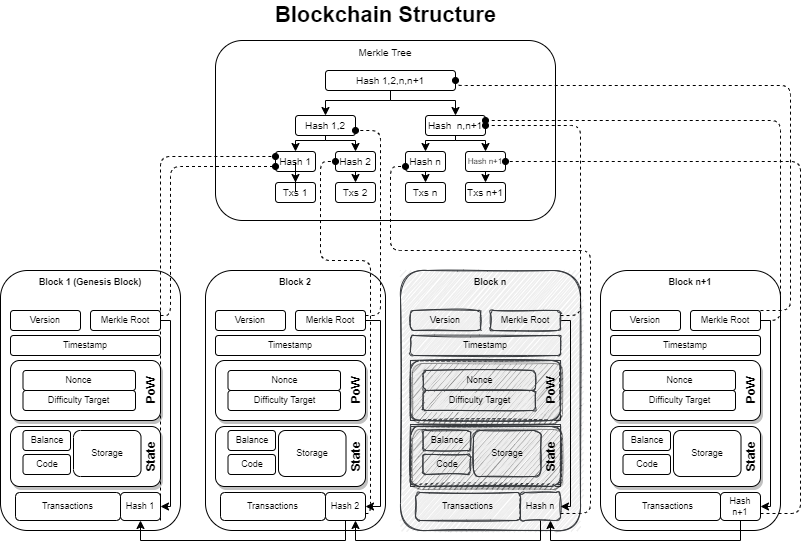
\includegraphics[width=180mm]{img/BlockchainStructure.png}
    \caption{Structure of a \ac{PoW} Blockchain ledger}
    \label{fig:BlockchainStructure}
\end{figure}

\subsection{Blockchain Ledger}
Figure \ref{fig:BlockchainStructure} shows the main components of a Blockchain structure which form the Ledger. This basic components are generated and validated by the different nodes in the System and later allow other users to interact and submit transactions to it. Depending of the type of blockchain different consensus mechanisms are generated in order to insert and validate the transactions block by block. 
The components of the ledger are:
\subsubsection{Block}
Represents a set of stored transactions submitted by different users and approved by node validators. To be able to insert data into a single block, certain rules have to apply: 
\begin{itemize}
    \item A user connected to the system and willing to insert data (submit a transaction) needs to prove its identity with a public and private key, which will allow him to interact with its asset in order to update the ledger by sensing or receiving (update or submit). Once the user and its ownership are properly identified and approved respectively, the transaction enters in a "data cache" where other transactions are waiting to be submitted in the ledger. There are several ways data can be validated and approved to be inserted into the ledger, but most commonly public Blockchains will request a transaction fee (paid in tokens) to commit the transaction. The fee allows the system to function as the machines in charge of maintaining and approving the transactions receive such value in exchange of the resources they use. Depending on the amount paid in the fee, the transaction will take or not priority to be inserted in the next block. Once the block reaches a certain size or time, it is generated, hashes and send to other peers.
\end{itemize}

\subsubsection{Version}
Indicates the version that the particular block uses. There are three types of Blockchain versions.

\begin{itemize}
    \item \emph{Version 1.0 (cryptocurrency)} ). It used a public ledger to store the data.
    \item \emph{Version 2.0 (Smart Contracts)} ). Indicates that embedded source code in the block has been executed for the generation of the block.
    \item \emph{Version 3.0 (\ac{DAPP}s )}. It is used to create a decentralized structure, such as the Tor Browser.
    \item \emph{Version 4.0 (Blockchain for Industry)}. Used to create a scalable, affordable blockchain network so that more people can make use of it.
\end{itemize}
 
\subsubsection{Timestamp}
Used as proof that the particular block is used at what instance of a time. It is also used as a parameter to verify the authenticity of a block.

\subsubsection{Consensus}
\label{consensus}
A consensus is a fault-tolerant mechanism used to achieve agreement on a single data value or a single state of the network among distributed processes or multi-agent systems. It allows all parties to participate democratically and enable equal rights to validate and insert data in the Blockchain.

There are different consensus mechanisms\cite{BlockchainConsensus:online}: 
\begin{itemize}
    \item \emph{\ac{PoW}}
    One party proves to another which verifies that a particular computational effort has been expended. Subsequently, verification can be accomplished with minimal effort on the part of the verifying party. By requiring some work from a service requester, such as processing time by a computer, it was initially conceived to deter denial-of-service attacks and other forms of network abuse. In Bitcoin, it is used as a consensus mechanism for a permissionless decentralized network in which miners compete to append blocks and issue new currency with a success probability proportional to the computational effort expended.  A key characteristic of proof-of-work schemes is their asymmetry\footnote{The work (computation) that must be moderately complex, yet feasible by a computer (prover) but simple to verify by the service provider (verifier)}. Its design contains a built-in incentive structure that rewards validators by allocating computational capacity to the network with value in the form of money.  \ac{PoW} algorithms aim to deter data manipulation by establishing considerable energy and hardware-control requirements, thus expending large amounts of resources in the process.
    
    \item \emph{\ac{PoS}}
    This method avoids the computational cost associated with proof-of-work schemes by selecting validators based on their holdings of the associated cryptocurrency. The validators are rewarded for adding transactions to the block. PoS secures a system by requiring validators to possess some blockchain tokens to mount an attack. Because PoW does not require complex mathematical calculations, it is more energy-efficient.
    
    \item \emph{\ac{PoET}}
    It is commonly used on a permissioned Blockchain. First, every node in the system must be identifiable and accepted into the network. Then, a standard certificate authority validates them. With PoET, the “timer” is different for each node. Each participant in the network is assigned a random amount of time to wait. The first participant to finish waiting gets to commit the following block to the blockchain.
    
    \item \emph{\ac{PoA}}
    It is a spin on \ac{PoS} consensus that addresses the risk of how participants in a network can value a stake. the consensus stakes the actual identities of the nodes in the system and aligns incentives by placing social capital at risk. A greater incentive is to act in the network's best interest if more of its net worth is lodged in a node, therefore  wealthier participants could go \ac{AWOL} as they can eat any financial loss they would receive for doing so. There also exist validation nodes,  which stake their reputation on the network. As compensation, validators are the only nodes allowed to validate blocks. By identifying validators, \ac{PoA} consensus becomes inherently centralized and best suited for private Blockchains and consortiums, such as a group of banks or insurance companies.

    \item \emph{\ac{BFT}}
    Allows distributed system to reach consensus (agreement on the same value) even when some of the nodes in the network fail to respond or respond with incorrect information. The objective is to safeguard against the system failures by employing collective decision making when it is both correct and misleading. It aims to reduce influence of the faulty nodes. \ac{BFT} is derived from Byzantine Generals’ Problem\footnote{The Byzantine Generals Problem is a term etched from the computer science description of a situation where involved parties must agree on a single strategy in order to avoid complete failure, but where some of the involved parties are corrupt and disseminating false information or are otherwise unreliable.}.
    
    
    \item \emph{\ac{PBFT}}
    Designed to work efficiently in asynchronous systems. It is optimized for low overhead time. Its goal was to solve many problems associated with already available \ac{BFT} solutions. It has a primary node and secondary nodes. These nodes work together to reach a consensus, making this system one of the solutions to the Byzantine Generals Problem. The maximum number of faulty/malicious nodes cannot be equal to or greater than one-third of the total nodes in the system.

    \item \emph{\ac{DAG}}
    A directed graph is a \ac{DAG} if and only if it can be topologically ordered, by arranging the vertices as a linear ordering that is consistent with all edge directions. To send a transaction, a node must validate two or more transactions that already took place. As more transactions are sent through the network, that system of checks and balances strengthens. The flow of data through this model allows the reduction of transactional fees, since they are approved as users contribute to the security of the network by confirming past transactions.

\end{itemize}


\subsubsection{\ac{Nonce}}
Is an arbitrary number that can be used just once in a cryptographic communication. Such number will never be repeated, and is the result that a machine has to come across in order to be the first on providing the hash of that number.

\subsubsection{Difficulty Target}
Is a measure of how difficult it is to mine a block in a blockchain for a particular cryptocurrency with \ac{PoW} consensus. A high cryptocurrency difficulty means it takes additional computing power to verify transactions entered on a blockchain—a process called mining.
\subsubsection{State}
It is a pointer that systems of the blockchain system independently hold their own copy of the blockchain, and the current known "state" is calculated by processing each transaction in order as it appears in the ledger. Transactions are bundled and delivered to each node in the form of a block. As new transactions are distributed throughout the network, they are independently verified and "processed" by each node.
\subsubsection{Transactions}
Continuously set of data being created or updated in the ledger. Contains relevant information about the digital assets or smart contract instructions to operate and change the ledger.
\subsubsection{Hash}
It is the process of transforming any given key or a string of characters into a new value through the process of hashing. Shorter, fixed-length values can be represented by keys that enable finding and using the original data. A hash function generates new values according to a mathematical algorithm.. To prevent the conversion of hash back into the original key, a good hash always uses a one-way hashing algorithm.

\subsubsection{Merkle Tree}

Hash trees or Merkle trees are trees in which every leaf (node) is labelled with a cryptographic hash of a data block. The cryptographic hash of each inner node's label is included in its label. It allows efficient and secure verification of the contents of large data structures. Hash trees are a combination of hash lists and hash chains.


\subsection{Additional generalities}
All these components are basic to most of the Blockchain systems, regarding how nodes are assembled into the network depend mostly on the consensus mechanism adopted. for the purpose of this work the consensus aforementioned were deeply studied and incorporated in the proposal solution as it will be shown in the next sections.
%!TEX root = ../../main.tex
\subsection{Smart Contracts}
\label{ch:approach:intro:smartcontracts}

There is one specific technology created by the Ethereum Foundation which allowed for the first time the embedding of source code into the Blockchain called \emph{smart contract}.

A smart contract is a piece of structured code embedded into the Blockchain; it uses an \ac{API} to interact with the chain. Once in a block, it cannot be altered, but new versions and improvements can be reinserted. There is an implicit economical cost for submitting intelligent contracts into the chain and executing functions that will generate new blocks. Anyone willing to participate and be part of the contract must be a member of a \ac{DAO} or \ac{DAC}, use a public and key as a unique identity and a private key to sign the transaction being submitted. Generally speaking, smart contracts are public and can be easily visualized to know the conditions and rules that the involved parties will use to interact. Ethereum Network was the first blockchain to implement the generation and execution of Smart Contracts fully. 

In the white paper \cite{Ethereum30:online}, it stipulates the basis for the usage of \emph{Custom currencies} ans \emph{colored coins} (first integrated in the Bitcoin Blockchain) and how they can be extended to the usage of custom tokens coded in a \emph{Turing Complete}\footnote{A concept named after English mathematician and computer scientist Alan Turing- a system of data-manipulation rules (such as a computer's instruction set, a programming language, or a cellular automaton) is said to be "Turing complete" or "computationally universal" if it can be used to simulate any Turing machine.} programming language.

Smart Contracts have proved to be flexible and adaptable to deploy applications where trust and decentralization is vital. The technology is relatively new. Since 2015 many organizations have joined forces to include new programming language in different sets of ledgers. For the \emph{Ethereum} Blockchain the standard language is known as \emph{Solidity}\cite{SolidityEthereum:online}. With the arrival of other Systems, new programming languages where created whereas others like the  \emph{Hyperledger Foundation} implement \emph{JavaScript}, \emph{Java}, \emph{Go} and \emph{Solidity as well}.

They also allowed the creation of \ac{DAO}s, where multiple parties could cooperate and collaborate in the benefit of the Blockchain ecosystem by agreeing on the rules that the smart contract was intended to execute depending on the conditions and situations the users will perform as a result of interacting with the \ac{DLT}.

This phenomenon called the attention of the industry for its potential to cooperate and create immutable database systems, but adapted to an anonymous and permissioned approach.

\subsubsection{Non-fungibility}
\ac{NFT}\footnote{An object is fungible when and if it is identical to others and thus can be replaced without any loss (mutual interchangeability). On the other hand, an object is non-fungible if it posses unique properties, making it unequal to others and thus of a different transactional value than their reciprocals.} in the blockchain brings tremendous possibilities to store value and a representation of physical or virtual objects. When the concept was exploited and implemented for the first time as a true standard in the Ethereum Environment\cite{EIP721No48:online}, \footnote{Ethereum is another decentralized open source blockchain with smart contract functionality embedded since its conception. Conceived in 2013, its creator extended the potential that Bitcoin had as a decentralized system to enable the generation of digital contracts.} the public realized of the potential the technology could have to generate value over the issuance of public certificates able to be verified by anyone to proof authenticity or ownership for predefined assets. 

Although \ac{NFT}s have skyrocketed from public Blockchains to demonstrate their potential with digital art (paintings, music, certification of authenticity, among others), little has been researched and implemented in the industry. But Non-fungibility has proven to be a key player for future technologies and mutual collaboration. Having a system with which companies can implicitly trust and collaborate offers tremendous possibilities for the development of knowledge and data protection.

\begin{figure}[h]
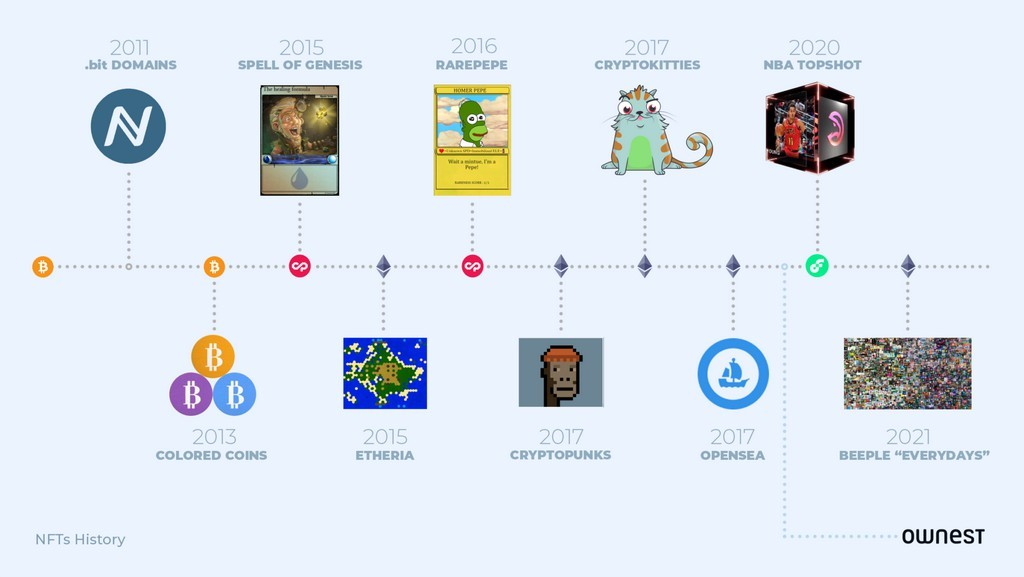
\includegraphics[width=15cm]{img/01-NFT_Timeline.png}
\centering
\caption{NFT Timeline, from the creation of Bitcoin domains, coloured coins to the new Ethereum and Altcoin derivatives  \cite{OwnestNF21:online}}
\end{figure}

Industries can nowadays benefit from blockchain systems to record and track data in more trustful ways and allow inter-entity cooperation. However, the problem of privacy, ownership, security and finance emerges when trying to implement such systems on a public blockchain. 

%!TEX root = ../../main.tex
\subsection{Hyperledger Fabric}
\label{ch:approach:intro:hyperledger}
Hyperledger Fabric is an open-source enterprise-grade permissioned \ac{DLT} platform designed for use in enterprise contexts that delivers crucial differentiating capabilities over other popular distributed ledger or blockchain platforms. It was established under the Linux Foundation and currently holds the solid support of enterprises and developers for continuous improvement. 
Important features:
\begin{itemize}
    \item Highly modular and configurable architecture, enabling innovation, versatility, and optimization for various industry use cases (banking, finance, insurance, healthcare, human resources, supply chain, digital music delivery, and others.).
    
    \item First distributed ledger platform to support chaincode\footnote{In Hyperledger Fabric Smart Contracts are bettern known as "chaincode"} authored in a general-purpose programming language (Java, Go, and Node.js), facilitating their development without learning a new language or \ac{DSL}.
    
    \item Permissioned platform. Unlike public permissionless networks, the participants are known to each other. While the participants may not fully trust one another (they may be competitors in the same industry), a network can be operated under a governance model built off what trust exists between participants, such as a legal agreement or framework for handling disputes.

    \item Support for pluggable consensus protocols enables the platform to be more effectively customized to fit particular use cases and trust models. By default, Fabric implements BFT consensus fully but could be modified instead for another  \ac{CFT} consensus protocol when fewer parties or organizations participate.

    \item Can leverage consensus protocols that do not require a native cryptocurrency to incent costly mining or fuel smart contract execution. Avoidance of a cryptocurrency reduces some significant risk/attack vectors, and the absence of cryptographic mining operations means that the platform can be deployed with roughly the exact operational cost as any other distributed system.

    \item Enables privacy and confidentiality of transactions and chaincode.

\end{itemize}
 
These differentiators make Fabric one of the better performing platforms available today regarding transaction processing and confirmation latency. 

\subsubsection{Hyperledger Fabric Components}

\begin{figure}[!h]
    \centering
    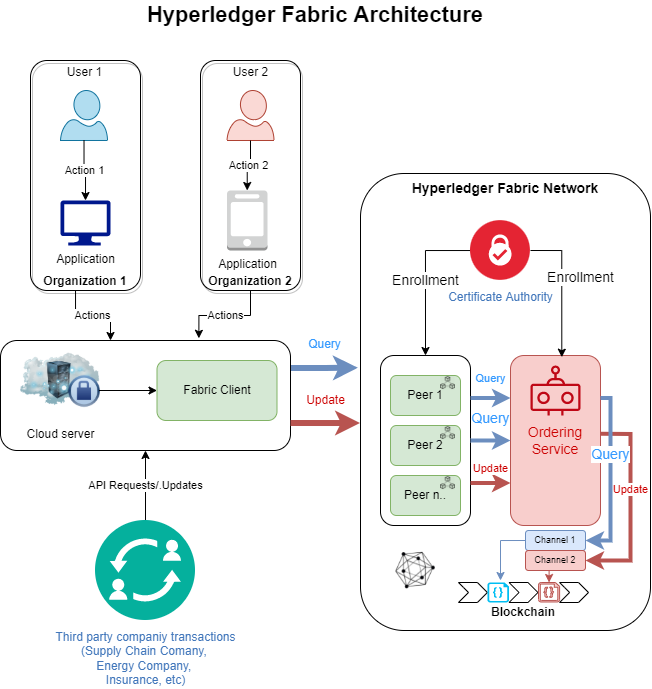
\includegraphics[width=15cm]{img/Hyperledger_Architecture.png}
    \caption{Hyperledger Fabric Architecture}
    \label{fig:HyperledgerArchitecture}
\end{figure}

\begin{itemize}
\item \textbf{Organization}. Virtual representation of a company/organization. Can define the areas and users that the organization will allow to interact with the \ac{DLT} 
\item \textbf{User}. Defines the entity that will directly interact with the ledger via \emph{Fabric Client} through a \ac{PKI} provided by a \ac{CA}.
\item \textbf{Application}. Is a custom software used by the organization and able to communicate with the ledger. The application will communicate with the ledger by sending actions to the \emph{Fabric Client}.
\item \textbf{Cloud server}. Infrastructure that hosts and provides the \emph{Fabric Client} that can directly communicate with the ledger.
\item \textbf{Fabric Client}. Application built by Hyperledger or custom code able to send query or update instructions to the ledger by invoking chaincode functions.
\item \textbf{Third-party companies}. Other organizations with custom applications or network infrastructure can also communicate with \emph{Fabric client} whenever the \ac{CA} grants access to the ledger.
\item \textbf{Certificate Authority}. Authorization service provider which uses \ac{PKI}-based certificates to network member organizations and their users. Issues one root certificate to each member and one enrollment certificate to each authorized user.
\item \textbf{Peer}. Servers that host a copy of the blockchain. Peers belong to the Organizations, and different organizations can have more than zero peers. The peers are coordinated by the ordering service and some of them will be selected as endorsers to validate chaincode transactions.
\item \textbf{Ordering Service} is in charge of ordering the transactions. An orderer or set of orderer nodes form an ordering service. Because Fabric’s design relies on deterministic consensus algorithms, any block validated by the peer is guaranteed to be final and correct. This architecture promotes finality by separating the endorsement of chaincode execution (which happens at the peers) from ordering, which provides advantages in performance and scalability as it eliminates bottlenecks.
\item \textbf{Channel}. Is a private tunnel (subnet) of communication between one or more organizations through which the parties agree over one or more chaincode instructions. Whenever organizations join a party, no other external entity is able to see the interactions between then, ensuring external anonymity and inner transparency. Peers can join one or more channels. Each channel has its own chain of blocks.
\item \textbf{Blockchain}. Is the ledger of the infrastructure, it exists in the peers and communicates via a single channel.
\end{itemize}

\subsubsection{Hyperledger Fabric Workflow}
The following steps form part of a typical Fabric workflow configuration:
\begin{enumerate}
    \item A user invokes a chaincode execution through his application, which generates a transaction invocation. Client broadcasts the transaction invocation request to the Endorser peer
    \item The Endorser peer checks the Certificate to validate the transaction. If verification is approved,it simulates the transaction by generating a response with a read-write set. Afterwards endorses the generated response using its own certificate. If the transaction fails a rejection response is sent.
    \item The client receives the endorsed proposal responses from Endorsing Peers.
    \item The client now sends the approved transaction to the orderer peer for this to be properly ordered and be included in a block.
    \item The orderer node includes the transaction into a block.
    \item The orderer node broadcasts the generated block to all Peers (to both Endorsing Peers and Committing Peers) on the relevant channel. Then, each Peer ensures that each transaction in the received block was signed by the appropriate Endorsing Peers. These individual peers then update their local ledger with the latest block. Thus all the network gets the ledger synced.
    \item The Clients receive any subscribed events if any.
    
\end{enumerate}

\begin{figure}[!h]
    \centering
    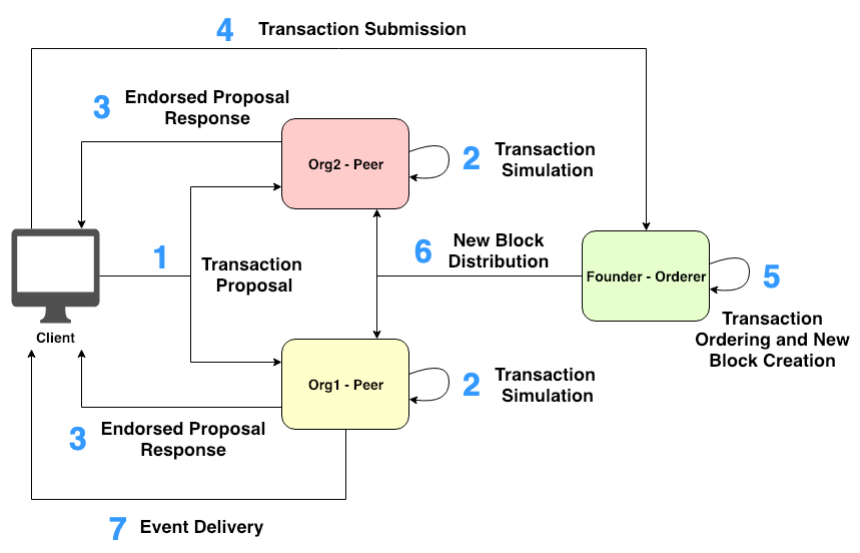
\includegraphics[width=15cm]{img/HyperledgerWorkflow.png}
    \caption{Hyperledger Fabric General Workflow}
    \label{fig:HyperledgerWorkflow}
\end{figure}
%!TEX root = ../../main.tex
\subsection{IPFS}
\label{ch:approach:intro:ipfs}

\ac{IPFS} is a distributed, \ac{P2P} file-sharing network enabling a high-scalability decentralized web\cite{benet2014ipfs}. Unlike common Internet sites that use location-based address, \ac{IPFS} stores information via content-based address and in the same manner as blockchain does, propagates the stored information in blocks to the connected peers. With this technology one can ensure that the stored data cannot be forged as the address is a \ac{CID}, which in essence is the root-hash of a Merkle Tree with additional metadata. Similar to blockchain systems, altering the information by even a single bit would drastically alter the hashing result.

\subsubsection{Properties}

\begin{itemize}
    \item  \ac{IPFS} is made up of all the connected nodes, which can store data and make it accessible to anyone requesting it.
    \item If a user requests a file, a copy of the file is cached on their node. The more different users request that data, the more cached copies will exist. Subsequent requests for that file can be fulfilled by any node or combination of nodes owning the file, preserving that way the stored information.
    \item  Because the data can be stored in pieces on many different computers, all those systems can feed parts of the data to its destination in parallel. This is intended to lower latency, reduce bandwidth, and avoid bottlenecks.
    \item As a result there is no focal point for hackers to attack.
    \item \ac{IPFS} also offers the possibility to submit encrypted data.
    \item Data is stored in chunks of 256 \ac{KB}, called \ac{IPFS} objects. Files larger than that are split into as many IPFS objects as it takes to accommodate the file. One IPFS object per file contains links to all of the other IPFS objects that make up that file.
    \item Once a file is added to the \ac{IPFS} network it is given a unique, 24-character hash \ac{CID}, which is the identifier within the network. Recalculating the hash when the file is retrieved verifies the integrity of the file. If the check fails, the file has been modified. 
    \item When files are legitimately updated, IPFS handles the versioning of files, meaning that new version of the file is stored along with the previous version. IPFS operates like a distributed file system, and this concept of versioning provides a degree of immutability to that file system.
    \item a Garbage collector will periodically remove cached \ac{IPFS} objects unless they are pinned to be preserved.
\end{itemize}

\begin{figure}[!h]
    \centering
    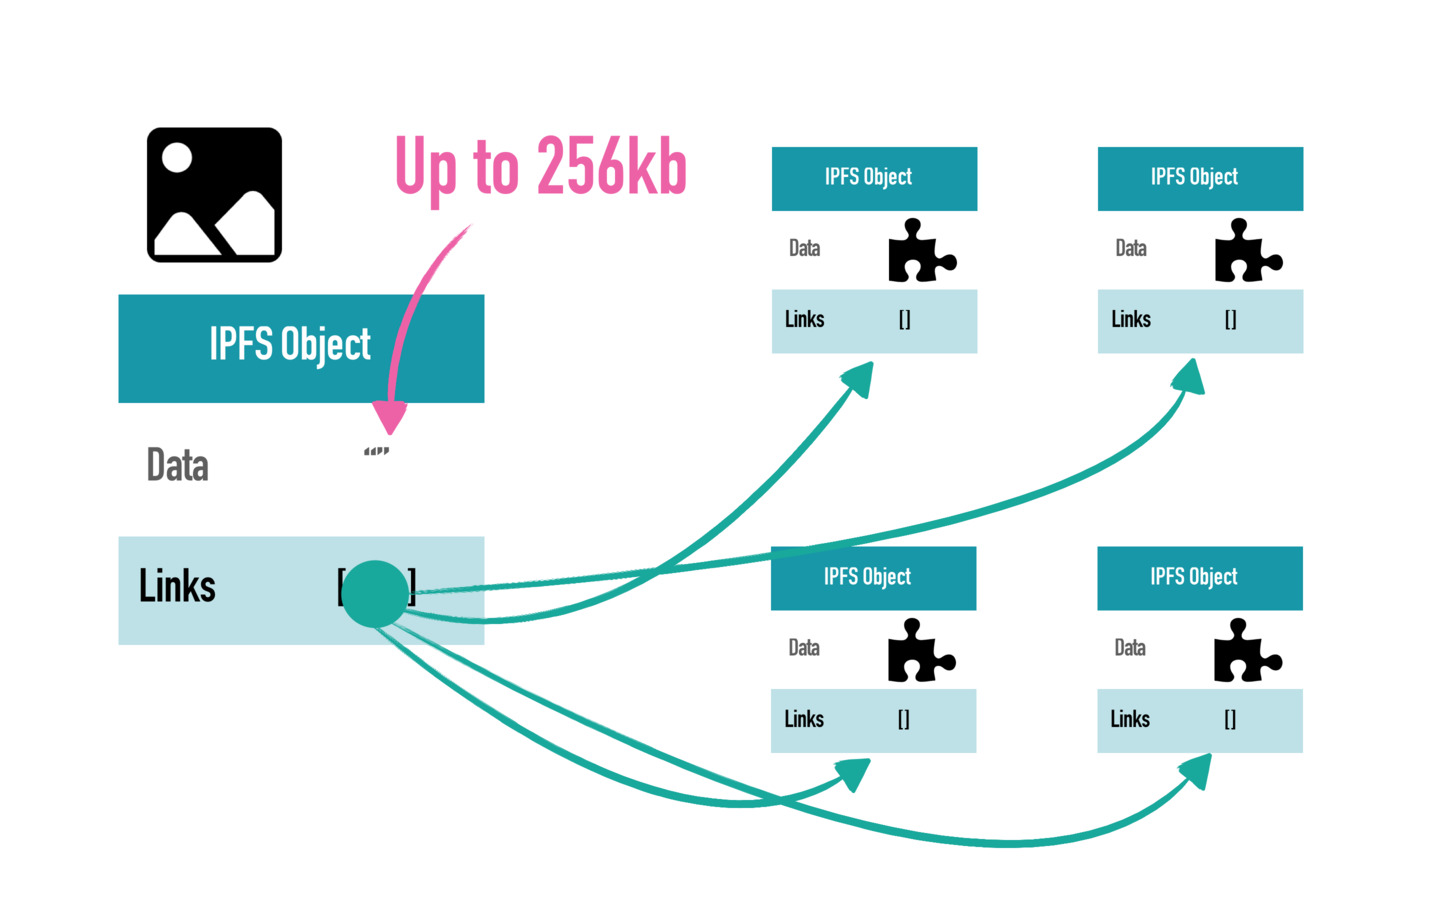
\includegraphics[width=15cm]{img/IPFSExample.png}
    \caption{A file being stored in the \ac{IPFS} network}
    \label{fig:IPFSExample}
\end{figure}


The properties of this \ac{DFS} provide meaningful advantages to work with Blockchain Systems since both work decentralized, trustless and in a set of hashed blocks.

%!TEX root = ../../main.tex
\section{Existing Approaches/Baselines}
All the components of the system aforementioned form the baseline for this thesis work, however little has been done in permissioned Blockchain systems that allow data management as a \ac{NFT} digital asset with \ac{IPFS}. There is however more research on its usage for public Blockchain networks and other industry purposes as the mentioned below. 


\subsubsection{e-Health}
Healthcare systems maintain electronic medical records using the centralized storage models, potentially compromising user privacy. Potential threats include unauthorized access to critical information such as identity details, diseases from which a patient suffers, and misuse of patients' data. \ac{IPFS} and blockchain technology, a distributed off-chain storage of medical data, can be created while preserving patient privacy.

\begin{itemize}
    \item \cite{9027313} proposes a framework to facilitate easy access to medical data by authorized entities while preserving consistency, integrity, and availability.
    
    \item \cite{CHEN2021102771} suggests a system able to handle \ac{EHR}s. for diabetes disease detection that provides an earlier detection of this disease by using various machine learning classification algorithms and securing the information. Blockchain, and \ac{IPFS} are used to collect patient's health information via wearable sensor devices.
    
    \item \cite{kumar2021decentralized} proposes in the same manner a decentralized system for medical data storage that allows the community to securely share information and remove it from central systems since the high cost of data breaches, cyber attacks and the implicit cost of restructuring the \ac{IT} infrastructure would prevent the progress in medical research and creation of new medical alternatives. 
    
    \item VAHAK\cite{9162738} is an interesting project aiming to provide a low-latency, secure and reliable infrastructure via Ethereum smart contracts, 5-G and \ac{IPFS} to allow communication and navigation of \ac{UAV}s and improve the air-distribution of medical supplies in areas hard to reach or in crisis.
    
    \item HealChain\cite{8865388} is a decentralized \ac{DMS} for Mobile Healthcare Using Consortium Blockchain, that aims to build a system where security prevails when patients share medical data wirelessly.
    
    \item \cite{9066212} is another system implementation to handle \ac{EHR} criptographically and decentralized.
    
    \item \cite{9759580} Has implemented a case study in Nepal for an Ethereum and \ac{IPFS} based Application model to record and share patient healdh information.
    
\end{itemize}

\subsubsection{Patents and intellectual property}
\begin{itemize}
    \item \cite{bamakan2022patents} intends to apply \ac{NFT}-based patent framework in public Blockchain networks and divers \ac{DFS}  to the intellectual property to promote transparency and liquidity for innovators willing to commercialize their inventions or be funded.
    
    \item \cite{agyekum2019digital} propose a digital media copyright and content protection using \ac{IPFS} and Blockchain to expedite traditional digital copyright solidification and rights which are time consuming and labor-intensive using Hyperledger Fabric and the management of digital fingerprints for patents, ensuring immutability and provenance.
    
    \item \cite{8591029} models a data Integrity and confidentiality framework using encryption, smart contracts and Apache Isis for the automatic audit trial. 
 
\end{itemize}

\subsubsection{Automotive}
\cite{nizamuddin2021blockchain} proposes an \ac{IPFS}/Ethereum blockchain-based system for the auto insurance sector to solve the problem of fraud and latency and bureaucracy that customers face whenever acquiring insurance for for vehicles. Insurance prevent the industry from progressing due to the liabilities and difficulties it presents in many situations to understand it.

\subsubsection{Identity and Authorization}
\cite{9240966} present a solution for Blockchain-based \ac{MPA} for Accessing IPFS Encrypted Data using Ethereum smart contracts and proxy re-encryption algorithms. It incorporates reputation mechanisms in the smart contracts to rate the oracles based on their malicious and non-malicious behaviors. Thus, this system can solve insider's attack problem by ensuring that a single authority or party is not acting alone. 

\subsubsection{Tourism}
\cite{demirel2021smart} have created a model with Blockchain and \ac{IPFS} integration for post pandemic economy for the tourism industry to fill the gap in the existing methods related to the use of the \ac{IoT}, devices with smart contracts without a need for intermediaries for the reservations and services secured by Blockchain. The authors have created a booking system with a unique smart contract between customers and hotels, including all services that a customer may need and elimination commission fees as well as reception costs.


\subsubsection{Agriculture}
\cite{8718621} have created a Blockchain-Based Soybean Traceability in Agricultural Supply Chain by  utilizing smart contracts to govern and control all interactions and transactions among all the participants involved within the supply chain ecosystem. All transactions are recorded and stored in the ledger with links to \ac{IPFS} and thus providing to all a high level of transparency and traceability into the supply chain ecosystem in a secure, trusted, reliable, and efficient manner.
%!TEX root = ../../main.tex
\section{Analysis}

Ever since the world has been interconnected over the Internet, malicious parties have intended to take advantage over their computational resources and digital assets. As technologies improve and the society evolves into a digital world, attacks become more sophisticated, frequent and devastating. It is increasing month by month in an exponential ways, compromising governments and companies systems and data. 

Such has been the risk and consequences of cyber attacks and data breaches that in 2021\cite{10DataBreaches:online}:
\begin{enumerate}
    \item On average a data breach costs up to 8.64 million \ac{USD}.
    \item Global Cybercrime costed over 6 trillion
    \item Businesses fell victim of ransomware every 11 seconds.
    \item Took up to 220 days to contain a data breach, with healthcare industry being the slowest to recover with over 320 days.
    \item  As more users perform remote works cybercriminals keep increasing their attacks over telecommuters and remote access pathways
    \item Properly containing a data breach could have saved up to 1 million \ac{USD} in less than 200 days
    \item More than 8\ac{TB} of data were leaked.
    \item A total of 270 major data breaches occurred, exposing 238 Million of records and 16 billion \ac{USD} per day.
\end{enumerate}

\begin{figure}[h]
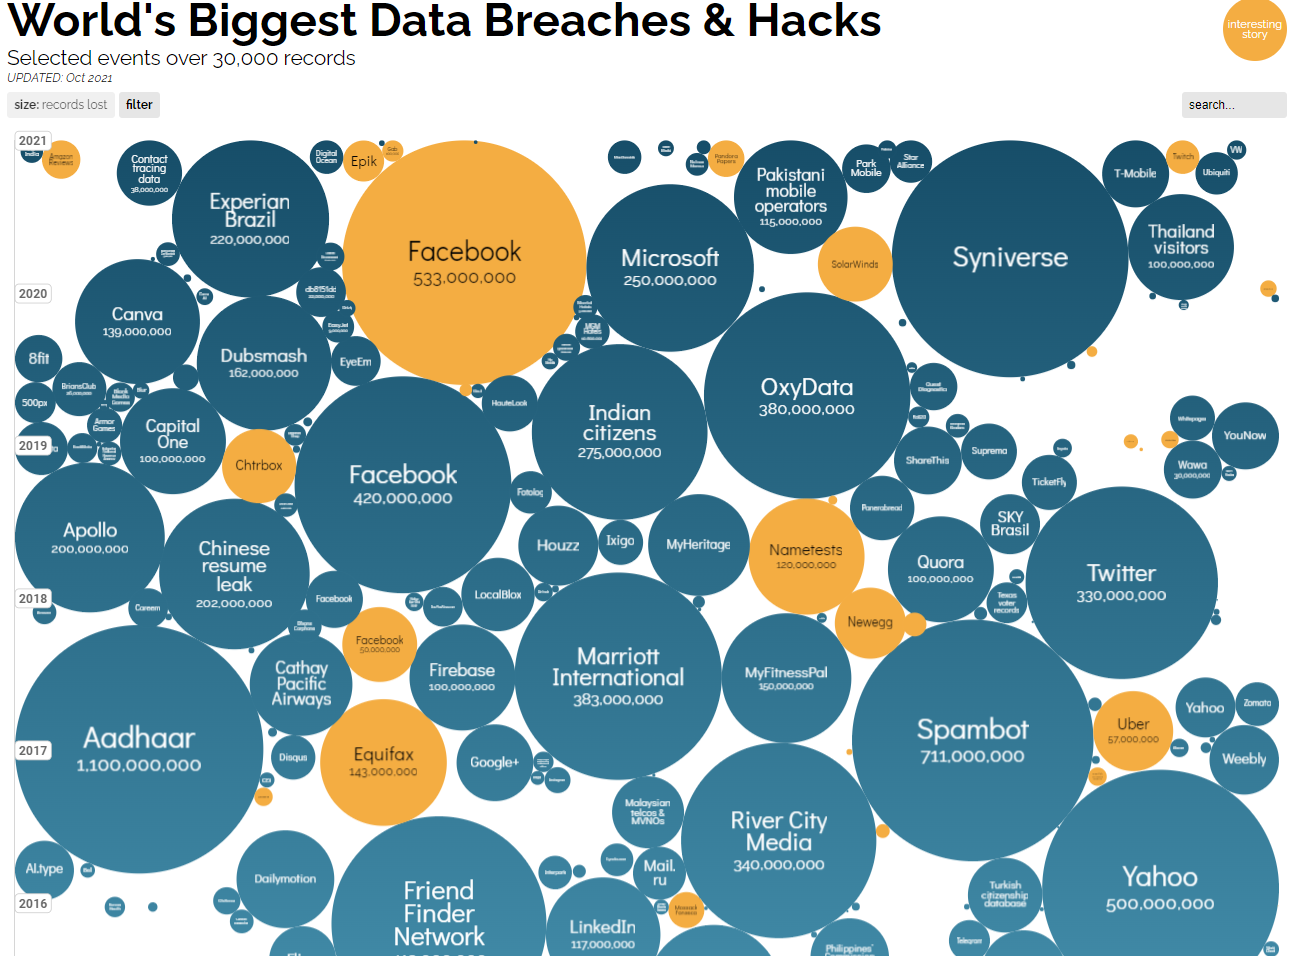
\includegraphics[width=15cm]{img/DataBreach.png}
s\caption{Word's Biggest data breaches and hacks occurred fro 2016 to October 2021  \cite{WorldDataBreach:online}}
\label{fig:worldDataBreach}
\end{figure}
Moreover, in 2021 several Nordic companies were victim of important cyber attacks ,peaking in December 2021\cite{Nordicco81:online}. Affected industries corresponded to the region’s largest industrial, food and  service providing sector.
Affected companies were Vestas, Wind Systems, Amedia, Nortura
and Nordic Choice Hotels

\begin{figure}[h]
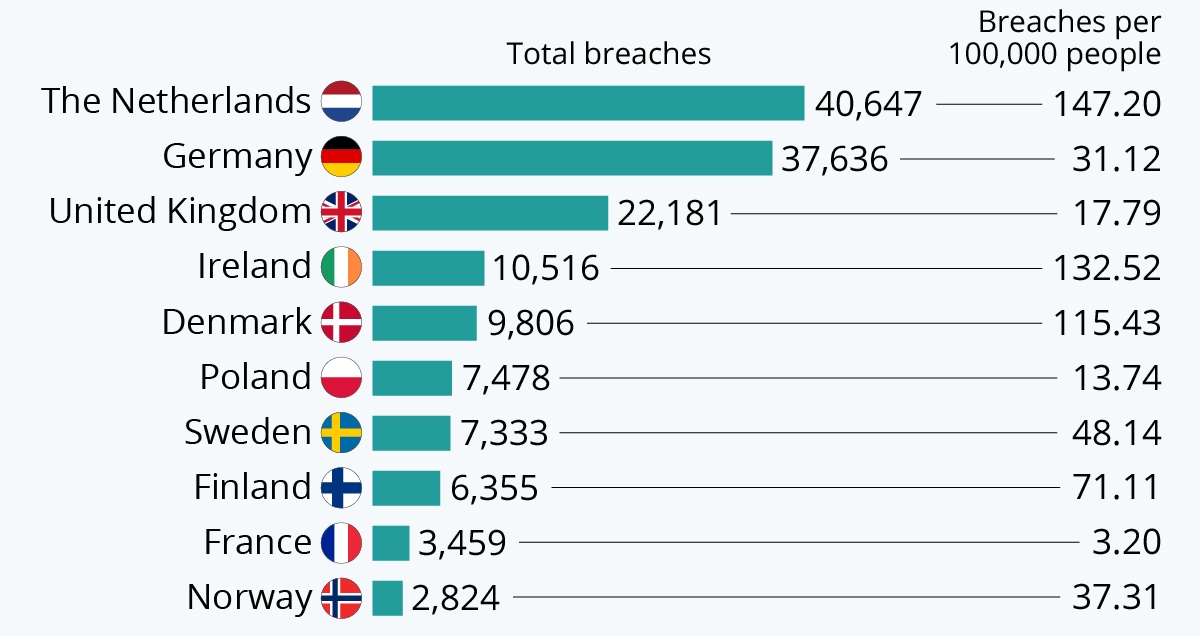
\includegraphics[width=15cm]{img/GDPRDataBreach.jpeg}
\centering
\caption{Top-10 \ac{GDPR}-per-country data breaches notified per \ac{EEA} jurisdiction from May 2018 to October 2020\cite{Statista:online}}
\end{figure}

It is clear that with the current resources (both human and digital) is impossible to overcome these threats. In addition data has become a vital asset. Companies are now legally liable to protect it and ensure that is properly protected with state of the art technologies. Failing to do that could lead them to bankruptcy or serious fines which in some cases could be of irrecoverable damage, lost of reputation or even catastrophic disasters for the society.


\subsubsection{Hypothesis}
\label{analysis_hyp}

With the implementation of a decentralized system in a Hyperledger Fabric and a chaincode implementing \ac{ERC}-721 standard with \ac{IPFS} network, it will be possible to manage and handle data between organizations in a safer and more secure way. Sharing information and ensuring that the non-repudation\footnote{Assurance that the sender of information is provided with proof of delivery and the recipient is provided with proof of the sender's identity, so neither can later deny having processed the information.} principle remains consistent over the network no matter how many parties or users join the infrastructure. 
%!TEX root = ../../main.tex
\section{Proposed Solution}
Having proposed the hypothesis to solve inter-organization data sharing and transmission through secure channels, the implementation of the system is shown in this section.

\subsubsection{System technologies}
The system gathers different technologies for the simulation 

\begin{figure}[!h]
    \centering
    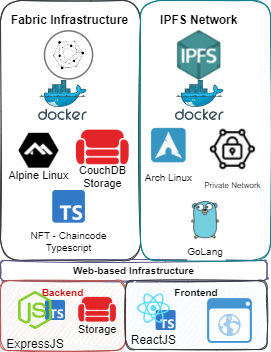
\includegraphics[scale=0.5]{img/System-Technologies.png}
    \caption{System technologies used}
    \label{fig:SystemTechUSed}
\end{figure}

\begin{itemize}
    \item \textbf{Docker}. Set of platform as a service products that use OS-level virtualization to deliver software in packages called containers.
    \item \textbf{Hyperledger Fabric version 2.2} is used in the system. It uses Docker technology to run and simulate the system. it uses \textbf{Alpine Linux} as the \ac{OS} repository.
    \item \textbf{Typescript}. A programming language superset of JavaScript developed and maintained by Microsoft. This code was used to develop the chaincode, back-end and front-end systems.
    \item \textbf{ExpressJS}. Back-end web application framework for Node.js designed for building web applications and APIs.
    \item \textbf{React}. Open-source front-end JavaScript library for building user interfaces based on UI components.
    \item \textbf{Apache CouchDB}. NoSQL document-oriented open-source database.
    \item \textbf{\ac{IPFS}}. Decentralized file storage system used content-addressed capabilities configured as a private network. It has been built in \textbf{GO} language and  \textbf{Alpine Linux} as \ac{OS}. Uses \textbf{Docker} containers as a base image.
\end{itemize}


\subsubsection{Proposed architecture}
The components configured and assembled to integrate the infrastructure work in a Docker system.

\begin{figure}[!h]
    \centering
    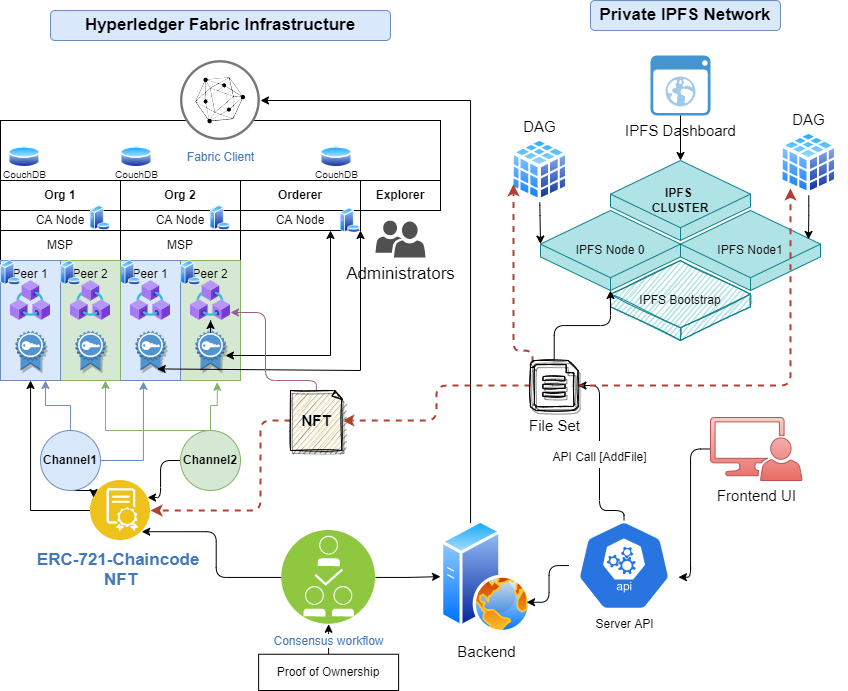
\includegraphics[width=15cm]{img/Hyperledger-NFT-Architecture.png}
    \caption{Proposed Architecture}
    \label{fig:SystemArch}
\end{figure}

\begin{itemize}
    \item \textbf{Hyperledger Fabric}. A a set of shell scripts and docker files assemble the required infrastructure to build the  \ac{DLT}. The Fabric infrastructure has the following subcomponents: 
    \begin{enumerate}
        \item Organizations. Two organizations have been created. One organizations is build primarily to simulate the minting process of a \ac{NFT} whereas the other can receive the minted token. The same process can also be made in the opposite way.
        \item Orderer node. Is the node in charge of sorting the transaction and creating the block. Once the block is created, it is forwarded to one of the organizations holding the Blockchain ledger. The orderer node does not hold a copy of the ledger but just coordinates and distributes the issued transactions.
        \item Orderer \ac{CA}. Is the node in charge of issuing and validating the certificates of the organizations and the wallet creation (based on the root certificates) for the users to interact with the system.
        \item Channel. Organizations in Hyperledger can join and interact through a private channel. The channel is previously known by the two organizations and they participate by having a server that holds a version of the ledger, a database server and a certificate authority server.
        \item Chaincode. The smart contract used to manage the ledger transaction and mint digital assets as \ac{NFT}s. The chaincode can be found in the appendix \ref{ERC271ChainCode}.
    \end{enumerate}
    \item \textbf{Private \ac{IPFS} network}. Consists of a set of Docker containers where each system holds a copy of the \ac{IPFS} file system.
    \begin{itemize}
        \item \ac{IPFS} bootstrap node. In the same way as the Ordered node receives the blocks of a transaction and transmits it to the organization nodes, it receives the file or data and transmits it to all the interconnected nodes, ensuring data persistence among the network.
        \item \ac{IPFS} Dashboard. It works as the \ac{UI} of the private network. Provides insights and data about the stored files and a preview of the data once a user can access through its content.
        \item \ac{IPFS} Nodes. Each organization can contribute to the system data repository by holding an \ac{IPFS} server.
    \end{itemize}
    \item \textbf{Back-end}. Server application that communicates with the Hyperledger network and extends its functionality by an API. 
    \begin{itemize}
        \item Connects organizations and corporate databases
        \item Communicates with the \ac{CA} servers to issue and hold certificates.
        \item Communicates with \ac{IPFS} private network API. 
        \item Holds a public \ac{REST} \ac{API} that provides all the functionality to register organizations, enroll users and mint \ac{NFT}s.
        \item Interacts with the Blockchain smart contract and retrieves the information contained in the ledger. 
    \end{itemize}
    \item \textbf{Front-end}. It serves as the \ac{UI} for user interaction. Allows the simulation of the system where any user can create an organization, enroll users, mint a \ac{NFT} and visualize them in the list.
\end{itemize} 


%!TEX root = ../main.tex

\chapter{Experimental Evaluation}
\label{ch:eval}

\section{Use case}
To simulate the system functionality a case for two persons from different organizations trying to issue and mint data, send it and making it available to one another.

\section{Experimental Setup and Data Set}
\subsection{Scenario}
Simulation of two organizations willing to share data with each other.
\subsubsection{Organization 1}
Represents an organization with important information gathered from external resources, expensive and difficult to obtain. Has the technology and infrastructure to generate data, but does not count with the know how neither infrastructure to process it or exploit it (similar to machine learning / big data scenarios).

\textbf{User 'Minter'}
"Organization 1" Creates a user "Minter" as a company representative in charge of submitting the data and creating a \ac{NFT} version of it inside the system. Then he can use the system to lend the data, enable a time frame visualization or transfer it.

\subsubsection{Organization 2}
Represents a technology company with skillful personal in data processing and domain area in the business of "Organization 1", but does not have the experience nor technology to gather it. Therefore it needs data from the aforementioned organization in order to create and expand their business.

\textbf{User 'Receiver'}
"Organization 2" Creates a user "Receiver"  as a company representative in charge of getting access to the \ac{NFT} minted data by "Organization 1" via user "Minter" which will be used as the data source to perform machine learning training operations. 

With the use of the NFT System framework these parties can cooperate and participate by trusting that the information is secure, has not been altered and can be easily verified by them and other parties.

\section{Experimental Results}
The complete simulation of the process is shown in this section.

\subsection{System registering and user enrollment}
The NFT system provides a friendly user interface to allow organizations to be registered into the Fabric network to use a specific channel. 
Prior to this process Fabric generated a \ac{CA} with which they can identify as trusted entities and fair participants of the network.

The first time an organization registers itself to join a private channel, an admin account is created. The admin account then is able to configure organization parameters and new users with restricted access or different mining/system-usage capabilities.
in the figure \ref{fig:SeqDiag_RegisterEnroll} can be visualized the process any organization will take to register itself as a valid participant with its corresponding representatives.

 \begin{figure}[!h]
        \centering
        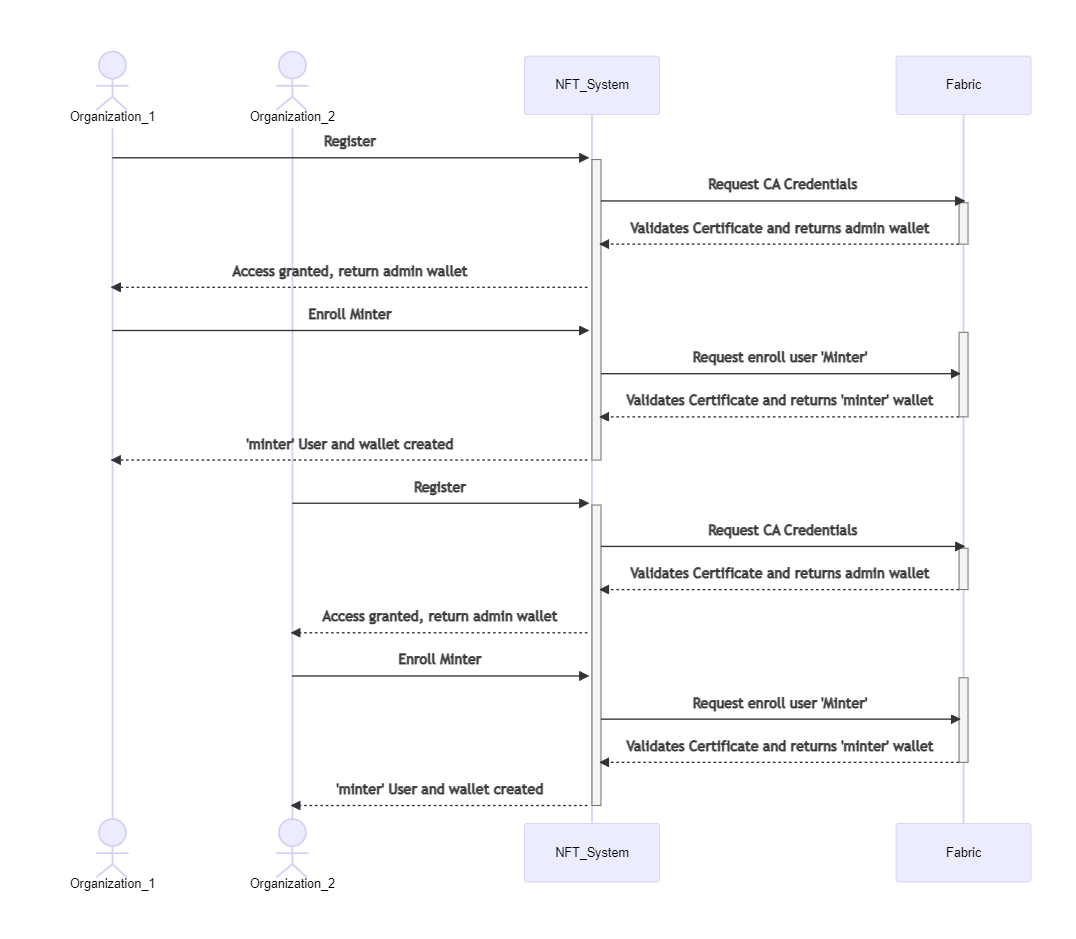
\includegraphics[width=15cm]{img/SequenceDiagram_RegisterEnroll.png}
        \caption{Sequence diagram of the Organization and user enrollment process in the system.}
        \label{fig:SeqDiag_RegisterEnroll}
    \end{figure}


 \begin{figure}[!h]
        \centering
        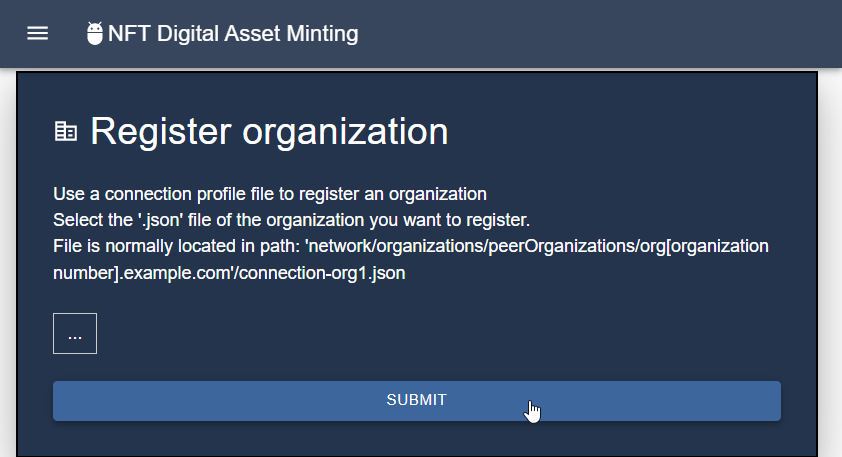
\includegraphics[width=7cm]{img/NFT_REGISTER.png}
        \caption{UI Register organization.}
        \label{fig:UI_Register}
    \end{figure}


 \begin{figure}[!h]
        \centering
        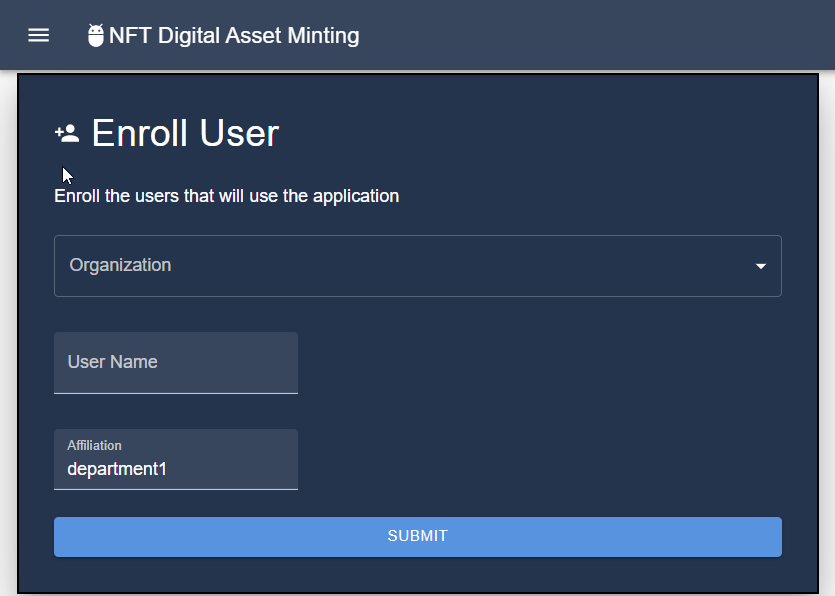
\includegraphics[width=7cm]{img/NFT_ENROLL.png}
        \caption{UI Enroll Users.}
        \label{fig:UI_Enroll}
    \end{figure}

\hfill \break

\subsection{NFT Minting and data reading access}
Once the organizations and users have been properly enrolled it the following steps must occur:
\begin{enumerate}
    \item Minter access to the platform and selects the "Mint 
    \ac{NFT} option.
    \item Minter selects a file and completes the form metadata.
    \item Minter clocks on "submit" button to create the token.
    \item The System talks verifies that the file does not exist yet by:
    \begin{itemize}
        \item Asking to add the data file to the \ac{IPFS} network
        \item Asking to Fabric if there is any token with the corresponding \ac{CID}
    \end{itemize}
    For any of those cases to be true, the token will not be generated and an error will be returned.
    \item Once everything is approved the token is stored in the \ac{DLT} with the corresponding file \ac{CID} generated.
    \item 'Minter' can now send the \ac{CID} or additional token information to 'Receiver'. Then receiver can pull such information from the infrastructure. Because of its unicity purposes 'Receiver' will not be able to counterfeit or take ownership of the data unless explicitly stipulated and agreed by both parties.
\end{enumerate}

 \begin{figure}[!h]
        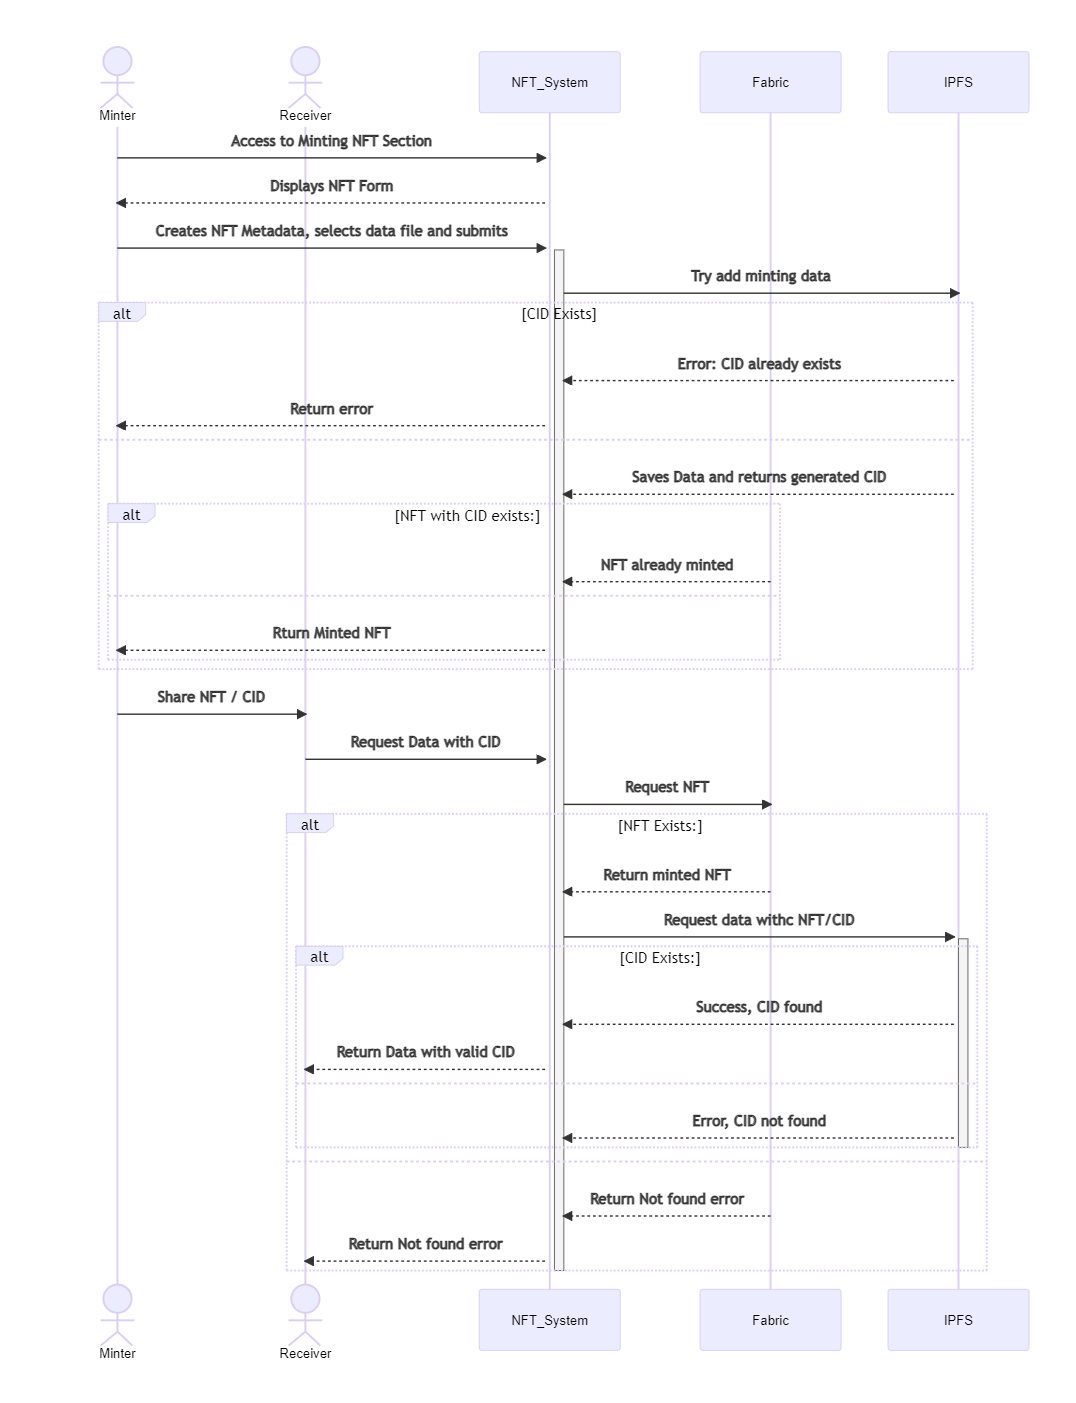
\includegraphics[width=15cm]{img/SequenceDiagram_MintNFT.png}
        \caption{Sequence diagram to mint a \ac{NFT}}
        \label{fig:SeqDiag_Mint}
    \end{figure}
    
 \begin{figure}[!h]
        \centering
        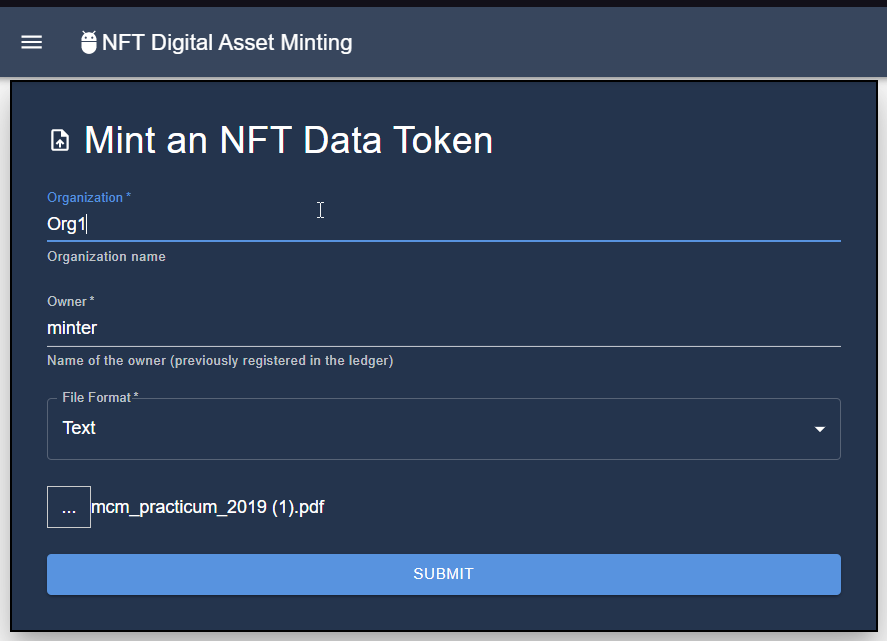
\includegraphics[width=10cm]{img/UIMinting.png}
        \caption{Front-end showing minting process.}
        \label{fig:UI_Mint}
    \end{figure}

 \begin{figure}[!h]
        \centering
        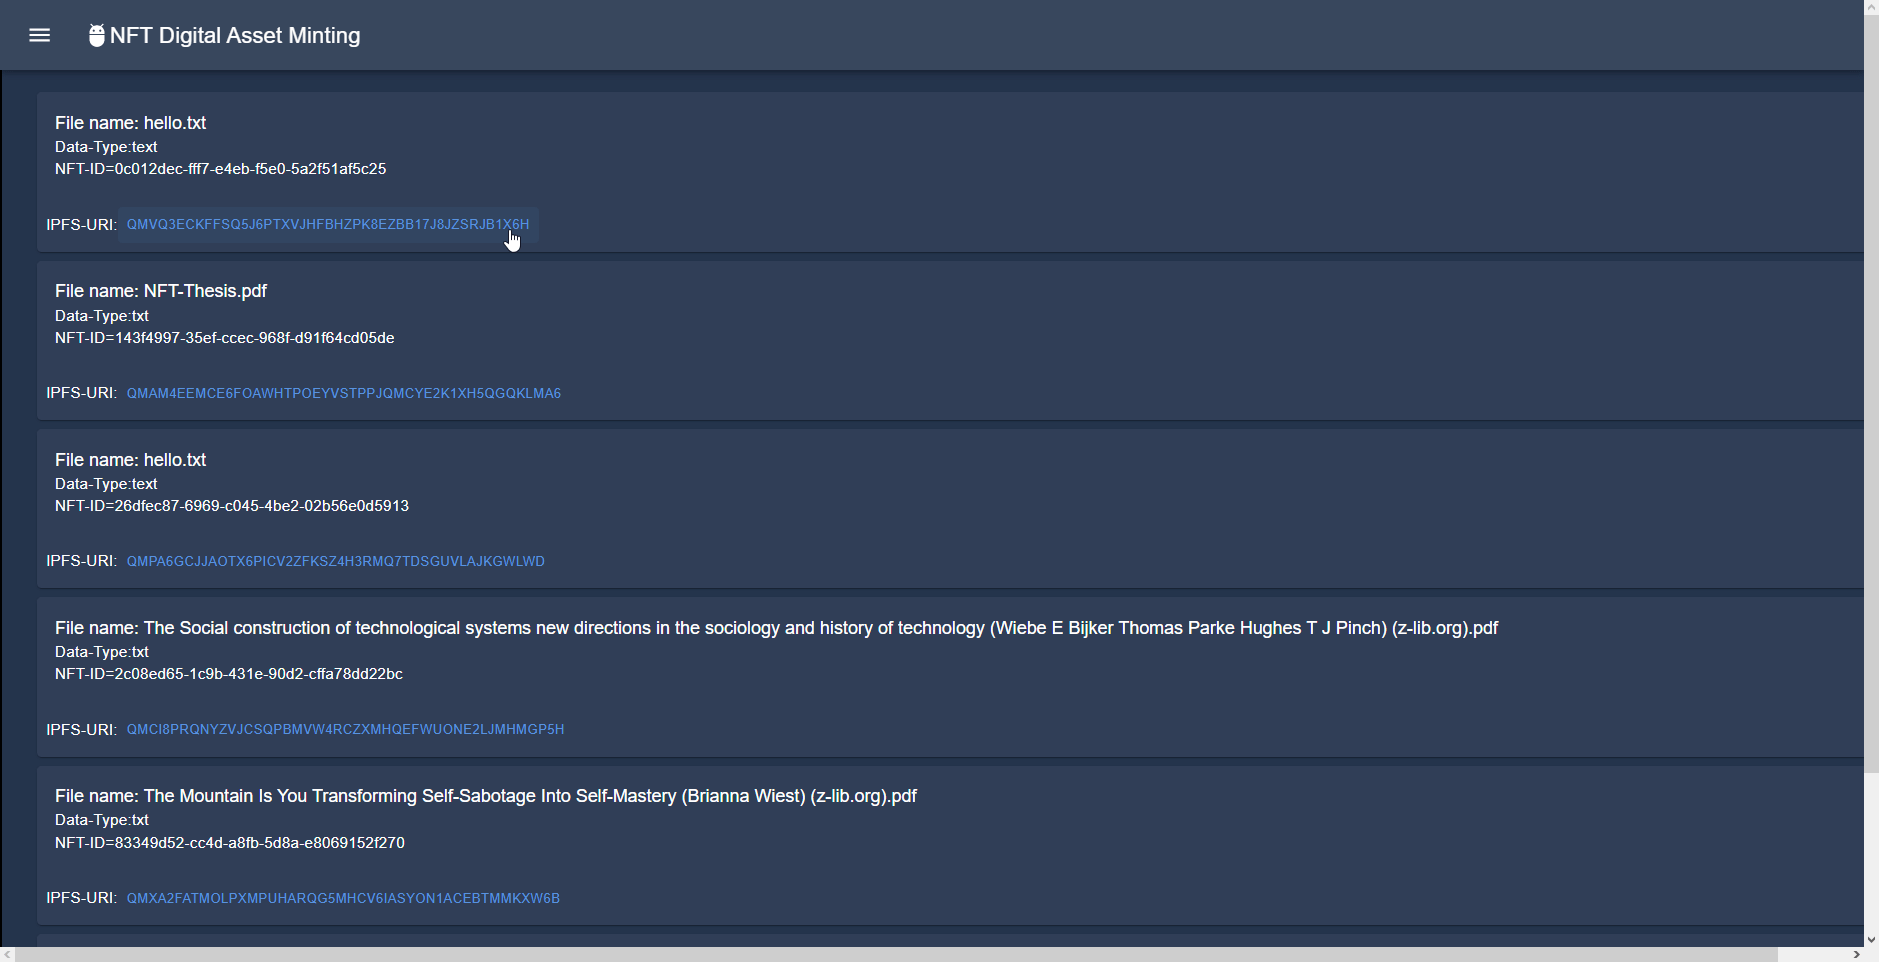
\includegraphics[width=15cm]{img/SystemList.png}
        \caption{Front-end showing minted \ac{NFT}s in the system.}
        \label{fig:UI_MintTokens}
    \end{figure}
    
\subsection{NFT Transfer}
It is possible through the \ac{REST} \ac{API} to transfer the generated tokens from one owner to the other. This process will acknowledge that the new user is the new owner of the \ac{NFT}. It is possible then to track the chain of ownership.

\subsection{NFT Burning}
The system also supports burning an \ac{NFT}, which basically blocks the token and flags it as unusable. if that happens, burned \ac{NFT} and \ac{CID} data cannot be accessed via the platform.

IT is possible, however to access the data via the \ac{IPFS} server.
%!TEX root = ../thesis.tex

\chapter{Discussion}
\label{ch:discussion}
The implementation of digital asset management through issuance of \ac{NFT}s represents a milestone in the generation of decentralized secure frameworks for industrial applications.

The implicit security of Blockchain with Hyperledger management and the privacy such technology offers will allow different organizations to participate and cooperate securely, but not anonymously. 

All parties will be able to acknowledge data ownership. If desired, data could be encrypted as well and managed trough additional smart contracts. In addition to this, \ac{IPFS} network is able to control, distribute and manage the added data as a \ac{DFS}. The final simulation of the environment allows testers, to acknowledge the workflow of the framework and further expand its capabilities in a modular way.

\section{Results}
The results of the built application indicate that it is potentially feasible to create decentralized systems specialized in data management and control for industrial purposes.
%!TEX root = ../thesis.tex

\chapter{Conclusions}
\label{ch:conclusion}

\section{Final comments}
In line with the original hypothesis stated in \ref{analysis_hyp} it is possible to confirm that the construction of decentralized systems is possible and will create yet unforeseen possibilities to manage information and provide:
\begin{itemize}
    \item System scalability
    \item Modularity
    \item Self Governance by smart contract agreement
    \item Privacy and security
    \item Mutual cooperation
\end{itemize}

Systems such as this can be governed or not by a central authority. Depending on the business needs and industrial purposes different scenarios could be developed and simulated.

Key findings through the research and development of this thesis project are:
\subsection{Blockchain and DLT}.
Data integrity and consistency safeguarding. Decentralized system nowadays allow very easily to verify data origin, integrity and non-repudation principle  establishes new ways of working and contributing for the development and research of technology.

\subsection{Security}
The created infrastructure has several layers of security and implicit elements to protect parties and their data from improperly accessing information. 
\subsubsection{\ac{CA}s}
Different parties can choose to rely over a central or multiple \ac{CA}s. As long as there is a common agreement previously established by smart contracts and common consensus, it will be possible to create highly resistant and resilient systems to malicious attacks. The modularity of Blockchain allows the cooperation of parties in benefit of the whole system, therefore rejecting undesirable or suspicious behaviour.

\subsubsection{Private channels}
Private channels in Hyperledger Fabric allow organizations to create a subsystem inside the framework, where sub smart contracts can be created to allow privacy between a single, two or more entities in different regions of the world.
Therefore, while every organization can hold a copy of the ledger and data, only those with the right privileges can be allowed to interact with the hidden rules.

\ac{IPFS} offers several layers of security, data can be encrypted and directed by smart contract instructions and even by the security layers set into the built system. 

\subsection{Governance}
Organizations can self in their best interest to preserve business functionality and choose the most suitable way to manage data. That being said, they will be able to choose which \ac{CA} is the best, what rules in the smart contract can be implemented and under which conditions entities can mint or transfer \ac{NFT}s.


\section{Future Work}
It is intended for anyone willing to extend and expand the functionality of this thesis work to move within the following points:
\subsection{System integration}
This thesis project can complement the work made by \cite{akbarAli}, which explains how shared data can be used to perform workflows for different purposes such as Big data analytics and Machine learning. One key advantage of this implementation relies on the fact that participants will have no direct access to shared data itself, but to a framework where it can be processed and manipulated to generate different models and insights. When connecting both systems, it will be possible to create and encapsulate information, self data encryption can grant that even different organizations own a copy of the blockchain and \ac{IPFS} network, they cannot read the information unless they do it directly from the proposed application.

\subsection{NFT and Smart Contract extension}
An extension of \ac{ERC}-721 smart contract implemented in \ref{ERC271ChainCode} can be easily extended to create new business rules such as:

\subsubsection{\ac{NFT} delegated ownership and transfer}
Not only one user, but multiple entities could possess a digital asset, sharing a percentage of such element. Therefore new rules can be suggested to interact, protect and manipulate information.

\subsubsection{Consensus}
New consensus mechanisms can be generated to incentivize the usage of the network. This project contains for example rules to rank information and create a reputation level for the organizations, which can increase the value of the minted \ac{NFT}. In other scenarios can be possible to create digital ownership by data origin, geographical location and mechanisms of burning so it cannot be used by other parties.
 
\subsubsection{Economics through Tokenization}
A very interesting approach to explore is the creation of economic tokens integrated with the \ac{NFT} system. Such tokens and in the same form that \ac{ETH} does with the Ethereum platform, every piece of data can be linked to another unity of tokens where once transferred its value in tokens can be transferred as well. The token-value of data can increase as its ranking of "valuable information" increases, or organization reputation does.
Depending on those economic mechanisms, different companies could be able to generate royalties and incentivize the usage of the system. Furthermore.

\subsubsection{Multi-system integration}
Furthermore, this project can be integrated with other public Blockchain platforms, and allow the issuance or reading of  Ethereum smart contracts, enabling its execution in the internal network. The possibilities are endless and adaptable to specific business needs.
%-----------------------------------------------------------------
% Now begin the Appendices, including them as separate files

\listoffigures
% \listoftables

\appendix
%!TEX root = ../main.tex
\chapter{Code and Instructions}
\label{apx:main}

\section{File repository}
\label{FileRep}
The repository with the code to download the system and perform the simulation is available at:
\url{https://github.com/asahicantu/NFT-Thesis}.

 \begin{figure}[!h]
        \centering
        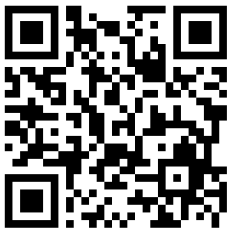
\includegraphics[width=5cm]{img/QrCode.png}
        \caption{Qr Code which will redirect to the Github Project stated in \ref{FileRep}}.
        \label{fig:QRCode}
\end{figure}

\section{Instructions to run the code}
To run the project follow the following steps:

\subsection{Prerequisites}
A Linux operating system or bash scripting shell is required.
On a windows machine the usage of \ac{WSL} (any Linux distribution) can help to run the project
Docker Desktop installed (if using Windows with \ac{WSL} make sure the option 'Use WSL 2 Based engine' or similar is selected).

\subsection{Run the application}
\begin{enumerate}
    \item Clone the repository
    \begin{lstlisting}[language=sh]
    git clone https://github.com/asahicantu/NFT-Thesis.git
    \end{lstlisting}
    \item Move to the repository's directory and then to the network directory
    \begin{lstlisting}[language=sh]
    cd NFT-Thesis/network
    \end{lstlisting}
    \item Enable execution mode for all .sh (shell scripting files)
    \begin{lstlisting}[language=sh]
    find . -name "*.sh" -exec chmod +x {} \;
    \end{lstlisting}
    \item Run the network infrastructure
    \begin{lstlisting}[language=sh]
    ./network start
    \end{lstlisting}
    \item Confirm no error occurred
     \begin{figure}[!h]
        \centering
        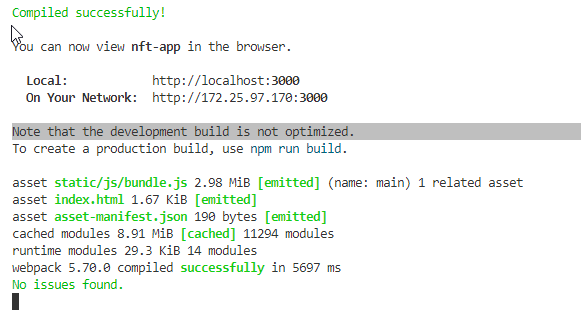
\includegraphics[width=10cm]{img/Client_Shell.png}
        \caption{Network shell showing successful run}.
        \label{fig:Network_Shell}
    \end{figure}
    \item Run server application in a different terminal
    \begin{lstlisting}[language=sh]
    cd ../web/server && npm install && npm run dev`
    \end{lstlisting}
    \item Confirm no error occurred
     \begin{figure}[!h]
        \centering
        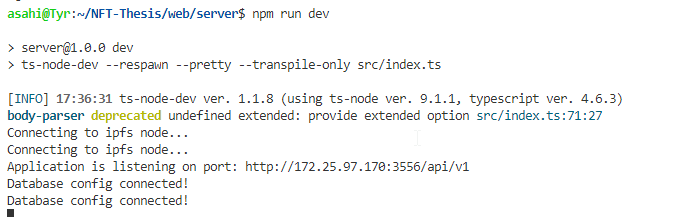
\includegraphics[width=10cm]{img/Server_Shell.png}
        \caption{Server shell showing successful run}.
        \label{fig:Server_Shell}
    \end{figure}
    \item Run web application in a different terminal
    \begin{lstlisting}[language=sh]
    cd ../client && npm install && npm run start`
    \end{lstlisting}
     \item Confirm no error occurred
     \begin{figure}[!h]
        \centering
        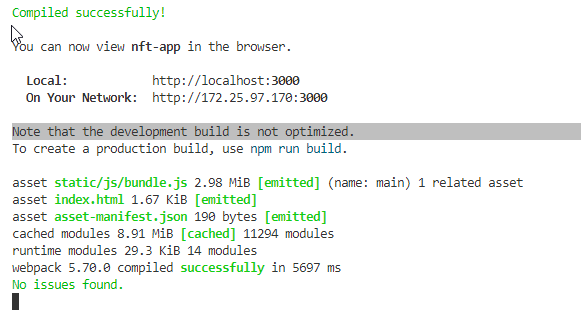
\includegraphics[width=10cm]{img/Client_Shell.png}
        \caption{Client shell showing successful run}.
        \label{fig:Client_Shell}
    \end{figure}
    \item Open the application in a web browser by using:
    \url{http://localhost:3000}.
    \item Confirm all steps were properly followed and no error occurred
     \begin{figure}[!h]
        \centering
        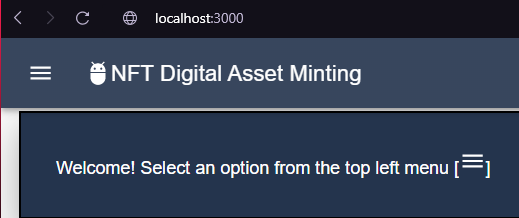
\includegraphics[width=10cm]{img/UI_MAIN.png}
        \caption{Main UI Page should be visible}.
        \label{fig:UI_MAIN}
\end{figure}

\end{enumerate}
\newpage
\section{NFT Chaincode}
This is the chaincode or smart contract implementing
\ac{ERC}-721 Standard in Hyperledger Fabric.
\textbf{File name:} tokenERC721Contract.ts
\label{ERC271ChainCode}
\begin{lstlisting}
/*
SPDX-License-Identifier: Apache-2.0
*/
import { Context, Contract, Info, Transaction } from 'fabric-contract-api'
import { NFT } from 'common/nft'
import KV from './@types/KV'

@Info({ title: 'TokenERC721Contract', description: 'ERC721 SmartContract, implemented in TypeScript' })
export class TokenERC721Contract extends Contract {
    // Define objectType names for prefix
    balancePrefix: string = 'balance'
    nftPrefix: string = 'nft'
    uriPrefix: string = 'uri'
    approvalPrefix: string = 'approval'
    // Define key names for options
    nameKey: string = 'name'
    symbolKey: string = 'symbol'

    constructor() {
        super('TokenERC721Contract')
    }

    @Transaction(false)
    public async setLogLevel(ctx: Context, loglevel: string): Promise < void> {
        const logger = ctx.logger.setLevel(loglevel)
    }

    /**
    *
    * @param {Context} ctx the transaction context
    * @returns {Number} The number of non-fungible tokens present in the ledger
    */
    @Transaction(true)
    public async GetAllResults(ctx: Context, isHistory: boolean, owner: string): Promise<any> {
        const iterator = await ctx.stub.getStateByPartialCompositeKey(this.balancePrefix, [owner])
        let allResults = []
        let res = await iterator.next() as any
        while (!res.done) {
            if (res.value && res.value.value.toString()) {
                let jsonRes: any = {}
                console.log(res.value.value.toString('utf8'))
                if (isHistory && isHistory === true) {
                    jsonRes.TxId = res.value.txId
                    jsonRes.Timestamp = res.value.timestamp
                    try {
                        jsonRes.Value = JSON.parse(res.value.value.toString('utf8'))
                    } catch (err) {
                        console.log(err)
                        jsonRes.Value = res.value.value.toString('utf8')
                    }
                } else {
                    jsonRes.Key = res.value.key
                    try {
                        jsonRes.Record = JSON.parse(res.value.value.toString('utf8'))
                    } catch (err) {
                        console.log(err)
                        jsonRes.Record = res.value.value.toString('utf8')
                    }
                }
                allResults.push(jsonRes)
            }
            res = await iterator.next()
        }
        iterator.close()
        return allResults
    }

    /**
     * BalanceOf counts all non-fungible tokens assigned to an owner
     *
     * @param {Context} ctx the transaction context
     * @param {String} owner An owner for whom to query the balance
     * @returns {Number} The number of non-fungible tokens owned by the owner, possibly zero
     */
    @Transaction(false)
    public async BalanceOf(ctx: Context, owner: string): Promise<number> {
        // There is a key record for every non-fungible token in the format of balancePrefix.owner.tokenId.
        // BalanceOf() queries for and counts all records matching balancePrefix.owner.*
        const iterator = await ctx.stub.getStateByPartialCompositeKey(this.balancePrefix, [owner])

        // Count the number of returned composite keys
        let balance = 0
        let result = await iterator.next()
        while (!result.done) {
            balance++
            result = await iterator.next()
        }
        return balance
    }

    /**
     * OwnerOf finds the owner of a non-fungible token
     *
     * @param {Context} ctx the transaction context
     * @param {String} tokenId The identifier for a non-fungible token
     * @returns {String} Return the owner of the non-fungible token
     */
    @Transaction(false)
    public async OwnerOf(ctx: Context, tokenId: string): Promise<string> {
        const nft = await this._readNFT(ctx, tokenId)
        const owner = nft.Owner
        if (!owner) {
            throw new Error('No owner is assigned to this token')
        }
        return owner
    }

    /**
     * TransferFrom transfers the ownership of a non-fungible token
     * from one owner to another owner
     *
     * @param {Context} ctx the transaction context
     * @param {String} from The current owner of the non-fungible token
     * @param {String} to The new owner
     * @param {String} tokenId the non-fungible token to transfer
     * @returns {Boolean} Return whether the transfer was successful or not
     */
    @Transaction(true)
    public async TransferFrom(ctx: Context, from: string, to: string, tokenId: string): Promise<boolean> {
        const sender = ctx.clientIdentity.getID()

        const nft = await this._readNFT(ctx, tokenId)

        // Check if the sender is the current owner, an authorized operator,
        // or the approved client for this non-fungible token.
        const owner = nft.Owner
        const approved = nft.ApprovedForTransfer == to
        const operatorApproval = await this.IsApprovedForAll(ctx, owner, sender)
        if (owner !== sender && !approved && !operatorApproval) {
            throw new Error('The sender is not allowed to transfer the non-fungible token')
        }

        // Check if `from` is the current owner
        if (owner !== from) {
            throw new Error('The from is not the current owner.')
        }

        // Clear the approved client for this non-fungible token
        nft.ApprovedForTransfer = undefined

        // Overwrite a non-fungible token to assign a new owner.
        nft.Owner = to
        const nftKey = ctx.stub.createCompositeKey(this.nftPrefix, [tokenId])
        await ctx.stub.putState(nftKey, Buffer.from(JSON.stringify(nft)))

        // Remove a composite key from the balance of the current owner
        const balanceKeyFrom = ctx.stub.createCompositeKey(this.balancePrefix, [from, tokenId])
        await ctx.stub.deleteState(balanceKeyFrom)

        // Save a composite key to count the balance of a new owner
        const balanceKeyTo = ctx.stub.createCompositeKey(this.balancePrefix, [to, tokenId])
        await ctx.stub.putState(balanceKeyTo, Buffer.from('\u0000'))

        // Emit the Transfer event
        const tokenIdInt = parseInt(tokenId)
        const transferEvent = { from: from, to: to, tokenId: tokenIdInt }
        ctx.stub.setEvent('Transfer', Buffer.from(JSON.stringify(transferEvent)))

        return true
    }

    /**
     * Approve changes or reaffirms the approved client for a non-fungible token
     *
     * @param {Context} ctx the transaction context
     * @param {String} approved The new approved client
     * @param {String} tokenId the non-fungible token to approve
     * @returns {Boolean} Return whether the approval was successful or not
     */
    @Transaction(true)
    public async Approve(ctx: Context, approved: string, tokenId: string): Promise<boolean> {
        const sender = ctx.clientIdentity.getID()

        const nft = await this._readNFT(ctx, tokenId)

        // Check if the sender is the current owner of the non-fungible token
        // or an authorized operator of the current owner
        const owner = nft.Owner
        const operatorApproval = await this.IsApprovedForAll(ctx, owner, sender)
        if (owner !== sender && !operatorApproval) {
            throw new Error('The sender is not the current owner nor an authorized operator')
        }

        // Update the approved client of the non-fungible token
        nft.ApprovedForTransfer = approved
        const nftKey = ctx.stub.createCompositeKey(this.nftPrefix, [tokenId])
        await ctx.stub.putState(nftKey, Buffer.from(JSON.stringify(nft)))

        // Emit the Approval event
        const tokenIdInt = parseInt(tokenId)
        const approvalEvent = { owner: owner, approved: approved, tokenId: tokenIdInt }
        ctx.stub.setEvent('Approval', Buffer.from(JSON.stringify(approvalEvent)))

        return true
    }

    /**
     * SetApprovalForAll enables or disables approval for a third party ("operator")
     * to manage all of message sender's assets
     *
     * @param {Context} ctx the transaction context
     * @param {String} operator A client to add to the set of authorized operators
     * @param {Boolean} approved True if the operator is approved, false to revoke approval
     * @returns {Boolean} Return whether the approval was successful or not
     */
    @Transaction(true)
    public async SetApprovalForAll(ctx: Context, operator: string, approved: boolean): Promise<boolean> {
        const sender = ctx.clientIdentity.getID()

        const approval = { owner: sender, operator: operator, approved: approved }
        const approvalKey = ctx.stub.createCompositeKey(this.approvalPrefix, [sender, operator])
        await ctx.stub.putState(approvalKey, Buffer.from(JSON.stringify(approval)))

        // Emit the ApprovalForAll event
        const approvalForAllEvent = { owner: sender, operator: operator, approved: approved }
        ctx.stub.setEvent('ApprovalForAll', Buffer.from(JSON.stringify(approvalForAllEvent)))

        return true
    }

    /**
     * GetApproved returns the approved client for a single non-fungible token
     *
     * @param {Context} ctx the transaction context
     * @param {String} tokenId the non-fungible token to find the approved client for
     * @returns {Object} Return the approved client for this non-fungible token, or null if there is none
     */
    @Transaction(false)
    public async GetApproved(ctx: Context, tokenId: string): Promise<string | object | undefined> {
        const nft = await this._readNFT(ctx, tokenId)
        return nft.ApprovedForTransfer
    }

    /**
     * IsApprovedForAll returns if a client is an authorized operator for another client
     *
     * @param {Context} ctx the transaction context
     * @param {String} owner The client that owns the non-fungible tokens
     * @param {String} operator The client that acts on behalf of the owner
     * @returns {Boolean} Return true if the operator is an approved operator for the owner, false otherwise
     */
    @Transaction(false)
    public async IsApprovedForAll(ctx: Context, owner: string, operator: string): Promise<boolean> {
        const approvalKey = ctx.stub.createCompositeKey(this.approvalPrefix, [owner, operator])
        const approvalBytes = await ctx.stub.getState(approvalKey)
        let approved
        if (approvalBytes && approvalBytes.length > 0) {
            const approval = JSON.parse(approvalBytes.toString())
            approved = approval.approved
        } else {
            approved = false
        }

        return approved
    }

    // ============== ERC721 metadata extension ===============

    /**
     * Name returns a descriptive name for a collection of non-fungible tokens in this contract
     *
     * @param {Context} ctx the transaction context
     * @returns {String} Returns the name of the token
     */
    @Transaction(false)
    public async Name(ctx: Context): Promise<string> {
        const nameAsBytes = await ctx.stub.getState(this.nameKey)
        return nameAsBytes.toString()
    }

    /**
     * Symbol returns an abbreviated name for non-fungible tokens in this contract.
     *
     * @param {Context} ctx the transaction context
     * @returns {String} Returns the symbol of the token
    */
    @Transaction(false)
    public async Symbol(ctx: Context): Promise<string> {
        const symbolAsBytes = await ctx.stub.getState(this.symbolKey)
        return symbolAsBytes.toString()
    }

    /**
     * TokenURI returns a distinct Uniform Resource Identifier (URI) for a given token.
     *
     * @param {Context} ctx the transaction context
     * @param {string} tokenId The identifier for a non-fungible token
     * @returns {String} Returns the URI of the token
    */
    @Transaction(false)
    public async TokenURI(ctx: Context, tokenId: string): Promise<string> {
        const nft = await this._readNFT(ctx, tokenId)
        return nft.URI
    }

    @Transaction(false)
    public async Token(ctx: Context, tokenId: string): Promise<NFT> {
        const nft = await this._readNFT(ctx, tokenId)
        return nft
    }
    /**
    * Tokens returns all non-fungible tokens assigned to an owner
    *
    * @param {Context} ctx the transaction context
    * @param {String} owner An owner for whom to query the balance
    * @returns {Array<any>>} The number of non-fungible tokens owned by the owner, possibly zero
    */
    @Transaction(false)
    public async Tokens(ctx:Context, owner: string): Promise<Array<NFT>> {
        let tokens = new Array<NFT>()
        // There is a key record for every non-fungible token in the format of balancePrefix.owner.tokenId.
        // TokensOf() queries for all records matching balancePrefix.owner.* and returns all of them
        const iterator = await ctx.stub.getStateByPartialCompositeKey(this.balancePrefix, [owner])
        let result = await iterator.next()
        while (!result.done) {
            //const nft = result
            //nfts.push(result.value)
            //ctx.logger.getLogger().log('INFO', result.value)
            //console.log(result.value)
            var val = result.value as KV
            const nftKey = ctx.stub.createCompositeKey(this.balancePrefix, [owner])
            var id = val.key.replace(nftKey,'')
            id = id.replace(/\u0000/g, '')
            let nft = await this._readNFT(ctx, id)
            tokens.push(nft)
            result = await iterator.next()
        }
        return tokens
    }

    @Transaction(false)
    public async TokenIds(ctx: Context, owner: string): Promise<Array<string>> {
        let tokenIds = new Array<string>()
        // There is a key record for every non-fungible token in the format of balancePrefix.owner.tokenId.
        // TokensOf() queries for all records matching balancePrefix.owner.* and returns all of them
        const iterator = await ctx.stub.getStateByPartialCompositeKey(this.balancePrefix, [owner])
        let result = await iterator.next()
        while (!result.done) {
            var val = result.value as KV
            tokenIds.push(val.key)
            result = await iterator.next()
        }
        return tokenIds
    }

    @Transaction(true)
    public async Rate(ctx: Context, tokenId: string, organization: string,rank:string): Promise<NFT> {
        const nft = await this._readNFT(ctx, tokenId)
        if (!nft.RankerOrganizations.includes(organization)) {
            nft.RankerOrganizations.push(organization)
            let rankInt = parseInt(rank)
            nft.Weight = (rankInt / 5  * nft.Weight )
        }
        return nft
    }

    // ============== ERC721 enumeration extension ===============
    /**
     * TotalSupply counts non-fungible tokens tracked by this contract.
     *
     * @param {Context} ctx the transaction context
     * @returns {Array<NFT>} Returns a count of valid non-fungible tokens tracked by this contract,
     * where each one of them has an assigned and queryable owner.
     */
    @Transaction(false)
    public async TotalSupply(ctx: Context): Promise<Array<NFT>> {
        // There is a key record for every non-fungible token in the format of nftPrefix.tokenId.
        // TotalSupply() queries for and counts all records matching nftPrefix.*
        const iterator = await ctx.stub.getStateByPartialCompositeKey(this.nftPrefix, [])
        let results = []
        // Count the number of returned composite keys
        let result = await iterator.next()
        while (!result.done) {
            if (result.value) {
                var nft = JSON.parse(result.value.value.toString()) as NFT
                results.push(nft)
            }
            result = await iterator.next()
        }
        return results
    }
    /**
     * TotalSupplyCount counts non-fungible tokens tracked by this contract.
     *
     * @param {Context} ctx the transaction context
     * @returns {Number} Returns a count of valid non-fungible tokens tracked by this contract,
     * where each one of them has an assigned and queryable owner.
     */
    @Transaction(false)
    public async TotalSupplyCount(ctx: Context): Promise<number> {
        // There is a key record for every non-fungible token in the format of nftPrefix.tokenId.
        // TotalSupply() queries for and counts all records matching nftPrefix.*
        const iterator = await ctx.stub.getStateByPartialCompositeKey(this.nftPrefix, [])

        // Count the number of returned composite keys
        let totalSupply = 0
        let result = await iterator.next()
        while (!result.done) {
            totalSupply++
            result = await iterator.next()
        }
        return totalSupply
    }
    // ============== Extended Functions for this sample ===============

    /**
     * Set optional information for a token.
     *
     * @param {Context} ctx the transaction context
     * @param {String} name The name of the token
     * @param {String} symbol The symbol of the token
     */
    @Transaction(true)
    public async SetOption(ctx: Context, name: string, symbol: string): Promise<boolean> {

        // Check minter authorization - this sample assumes Org1 is the issuer with privilege to set the name and symbol
        const clientMSPID = ctx.clientIdentity.getMSPID()
        if (clientMSPID !== 'Org1MSP') {
            throw new Error('client is not authorized to set the name and symbol of the token')
        }
        await ctx.stub.putState(this.nameKey, Buffer.from(name))
        await ctx.stub.putState(this.symbolKey, Buffer.from(symbol))
       return true
    }

    /**
     * Mint a new non-fungible token
     *
     * @param {Context} ctx the transaction context
     * @param {String} tokenId Unique ID of the non-fungible token to be minted
     * @param {String} tokenURI URI containing metadata of the minted non-fungible token
     * @returns {Object} Return the non-fungible token object
    */

    @Transaction(true)
    public async Mint(ctx: Context, id: string, uri: string, format: string, owner: string, ownerOrg: string, filename: string,date:number): Promise<NFT> {

        // Check minter authorization - this sample assumes Org1 is the issuer with privilege to mint a new token
        const clientMSPID = ctx.clientIdentity.getMSPID()
        if (clientMSPID !== 'Org1MSP') {
            throw new Error('client is not authorized to mint new tokens')
        }

        // Check if the token to be minted does not exist
        let exists = await this._nftExistsById(ctx, id)
        if (exists) {
            throw new Error(`The token with Id ${id} is already minted.`)
        }
        exists = await this._nftExistsByUri(ctx, uri)
        if(exists){
            throw new Error(`The token with Uri ${uri} is already minted` )
        }
        const nftToken: NFT = {
            ID: id,
            URI: uri,
            FileFormat: format,
            Owner: owner,
            Organization: ownerOrg,
            FileName: filename,
            Weight: 0,
            ApprovedForTransfer: undefined,
            Date:date,
            RankerOrganizations: []
        }
        // Add a non-fungible token
        const nftKey = ctx.stub.createCompositeKey(this.nftPrefix, [nftToken.ID])
        await ctx.stub.putState(nftKey, Buffer.from(JSON.stringify(nftToken)))
        const uriKey = ctx.stub.createCompositeKey(this.uriPrefix, [nftToken.URI])
        await ctx.stub.putState(uriKey, Buffer.from(nftToken.ID))
        // A composite key would be balancePrefix.owner.tokenId, which enables partial
        // composite key query to find and count all records matching balance.owner.*
        // An empty value would represent a delete, so we simply insert the null character.
        const minter = ctx.clientIdentity.getID() // Get ID of submitting client identity
        const balanceKey = ctx.stub.createCompositeKey(this.balancePrefix, [minter, nftToken.ID])
        await ctx.stub.putState(balanceKey, Buffer.from('\u0000'))

        // Emit the Transfer event
        const transferEvent = { from: '0x0', to: minter, tokenId: nftToken.ID }
        ctx.stub.setEvent('Transfer', Buffer.from(JSON.stringify(transferEvent)))
        return nftToken
    }

    /**
     * Burn a non-fungible token
     *
     * @param {Context} ctx the transaction context
     * @param {String} tokenId Unique ID of a non-fungible token
     * @returns {Boolean} Return whether the burn was successful or not
     */
    @Transaction(true)
    public async Burn(ctx: Context, tokenId: string): Promise<boolean> {
        const owner = ctx.clientIdentity.getID()

        // Check if a caller is the owner of the non-fungible token
        const nft = await this._readNFT(ctx, tokenId)
        if (nft.Owner !== owner) {
            throw new Error(`Non-fungible token ${tokenId} is not owned by ${owner}`)
        }

        // Delete the token
        const nftKey = ctx.stub.createCompositeKey(this.nftPrefix, [tokenId])
        await ctx.stub.deleteState(nftKey)

        // Remove a composite key from the balance of the owner
        const balanceKey = ctx.stub.createCompositeKey(this.balancePrefix, [owner, tokenId])
        await ctx.stub.deleteState(balanceKey)

        // Emit the Transfer event
        const tokenIdInt = parseInt(tokenId)
        const transferEvent = { from: owner, to: '0x0', tokenId: tokenIdInt }
        ctx.stub.setEvent('Transfer', Buffer.from(JSON.stringify(transferEvent)))

        return true
    }

    /**
     * ClientAccountBalance returns the balance of the requesting client's account.
     * @param {Context} ctx the transaction context
     * @returns {Number} Returns the account balance
     */
    @Transaction(false)
    public async ClientAccountBalance(ctx: Context): Promise<number> {
        // Get ID of submitting client identity
        const clientAccountID = ctx.clientIdentity.getID()
        return this.BalanceOf(ctx, clientAccountID)
    }

    // ClientAccountID returns the id of the requesting client's account.
    // In this implementation, the client account ID is the clientId itself.
    // Users can use this function to get their own account id, which they can then give to others as the payment address
    @Transaction(false)
    public async ClientAccountID(ctx: Context): Promise<string> {
        // Get ID of submitting client identity
        const clientAccountID = ctx.clientIdentity.getID()
        return clientAccountID
    }

    private async _readNFT(ctx: Context, tokenId: string): Promise<NFT> {
        const nftKey = ctx.stub.createCompositeKey(this.nftPrefix, [tokenId])
        const nftBytes = await ctx.stub.getState(nftKey)
        if (!nftBytes || nftBytes.length === 0) {
            throw new Error(`The tokenId ${tokenId} is invalid. It does not exist`)
        }
        const nft = JSON.parse(nftBytes.toString())
        return nft as NFT
    }

    private async _nftExistsById(ctx: Context, tokenId: string): Promise<boolean> {
        const nftKeyId = ctx.stub.createCompositeKey(this.nftPrefix, [tokenId])
        const nftBytesById = await ctx.stub.getState(nftKeyId)
        return nftBytesById && nftBytesById.length > 0
    }

    private async _nftExistsByUri(ctx: Context, uri:string): Promise<boolean> {
        const nftKeyUri = ctx.stub.createCompositeKey(this.uriPrefix, [uri])
        const nftBytesByUri = await ctx.stub.getState(nftKeyUri)
        return nftBytesByUri && nftBytesByUri.length > 0
    }
}
\end{lstlisting}


%-----------------------------------------------------------------
 \backmatter
 \label{Bibliography}
 %\lhead{\emph{Bibliography}}
 % Change the left side page header to "Bibliography"
  \bibliographystyle{unsrtnat}  % Use the "unsrtnat" BibTeX style for formatting the Bibliography
  \bibliography{Bibliography}  % The references (bibliography) information are stored in the file named "Bibliography.bib"

\uisbackcover
\end{document}